\documentclass[11pt]{article}
\usepackage[a4paper,left=22mm,right=22mm,top=23mm,bottom=25mm]{geometry}
\usepackage{graphicx}
\usepackage{url}
\usepackage{hyperref}
\usepackage{amsmath}
\usepackage{fancyhdr}
\usepackage[utf8]{inputenc}
\hypersetup{colorlinks=true,linkcolor=blue,urlcolor=blue}

\begin{document}
\clubpenalty 10000
\widowpenalty 10000

\title{3. Experimentální hodnocení kvality algoritmů}
\author{Ladislav Martínek}
\date{}
\maketitle
 
\section{Zadání úlohy} 

\begin{itemize}
\item Prozkoumejte citlivost metod řešení \href{http://www.csc.kth.se/~viggo/wwwcompendium/node211.html#7374}{problému batohu} na parametry instancí generovaných generátorem náhodných instancí. Máte-li podezření na další závislosti, modifikujte zdrojový tvar generátoru.
\item Na základě zjištění navrhněte a proveďte experimentální vyhodnocení kvality řešení a výpočetní náročnosti
\item Zkoumejte zejména následující metody
\begin{enumerate}
\item hrubá síla (pokud z implementace není evidentní úplná necitlivost na vlastnosti instancí)
\item metoda větví a hranic, případně ve více variantách
\item dynamické programování (dekompozice podle ceny a/nebo hmotnosti). FPTAS algoritmus není nutné testovat, pouze pokud by bylo podezření na jiné chování, než DP
\item heuristika - poměr cena/váha
\end{enumerate}
\item Pozorujte zejména závislosti výpočetního času (případně počtu testovaných stavů) a rel. chyby (v případě heuristiky) na:
\begin{enumerate}
\item maximální váze věcí
\item maximální ceně věcí
\item poměru kapacity batohu k sumární váze
\item granularitě (pozor - zde si uvědomte smysl exponentu granularity)
\end{enumerate}
\item Doporučuje se zafixovat všechny parametry na konstantní hodnotu a vždy plynule měnit jeden parametr. Je nutné naměřit výsledky pro aspoň čtyři (opravdu minimálně) vhodně zvolené hodnoty parametru, jinak některé závislosti nebude možné vypozorovat.
\end{itemize}

\section{Rozbor řešení}\label{kap:1}
Pro určení a sledování citlivosti na různé instance problému jsem využil generátor náhodných instancí, u které lze nastavovat jednotlivé parametry. U instancí problému jsou nastavovány parametry jako granulalita, maximální cena, maximální váha a poměr sumární váhy ke kapacitě batohu. Pokusím se odhadnout chování algoritmů při změnách parametrů jednotlivých instancí. Tedy sledovat citlivost algoritmů na dané parametry. 
\subsection{Metoda hrubé síly}
Medota hrubé síly nebude v tomto experimentu zkoumána, protože je zřejmé, že pokaždé projde všechny instance a tedy vubec není citlivá na jiné parametry, kromě paramentru n, který ale již by prozkoumán v 1. a 2. úloze.


\subsection{Metoda větví a hranic (B\&B)} 
U této metody očekávám velkou čitlivost na poměr celkové váhy a kapacity batohu, dále by metody mohla ovlivnit granularita. Tato metoda nemá horní mez a proto její čas může narůst až na metody hrubé síly. 

\subsection{Metody dynamického programování (obě dekompozice)}
U dekompozic očekávám citlivost vždy na daný parametr. U dekompozice podle ceny tedy citlivost na maximální cenu a u dekompozice podle váhy na maximální váhu. 

\subsection{Řešení heuristikou poměr cena/váha}
Očekávám, že heuristická metoda bude datově citlivá a to především na paramentry jako poměr celkové váhy a kapacity batohu nebo granularita. Vliv maximální ceny a váhy neočekávám.




\section{Popis kostry algoritmu}\label{kap:2}
Všechny algoritmy a průběh experimentu, zůstali stejné jako v úloze 2. Byli pouze změněny soubory s instancemi, které byli vygenerovány před experimentem.


\section{Experimenty}
 
 
\begin{figure}
	\centering
    \begin{minipage}[c]{0.49\textwidth}
        \centering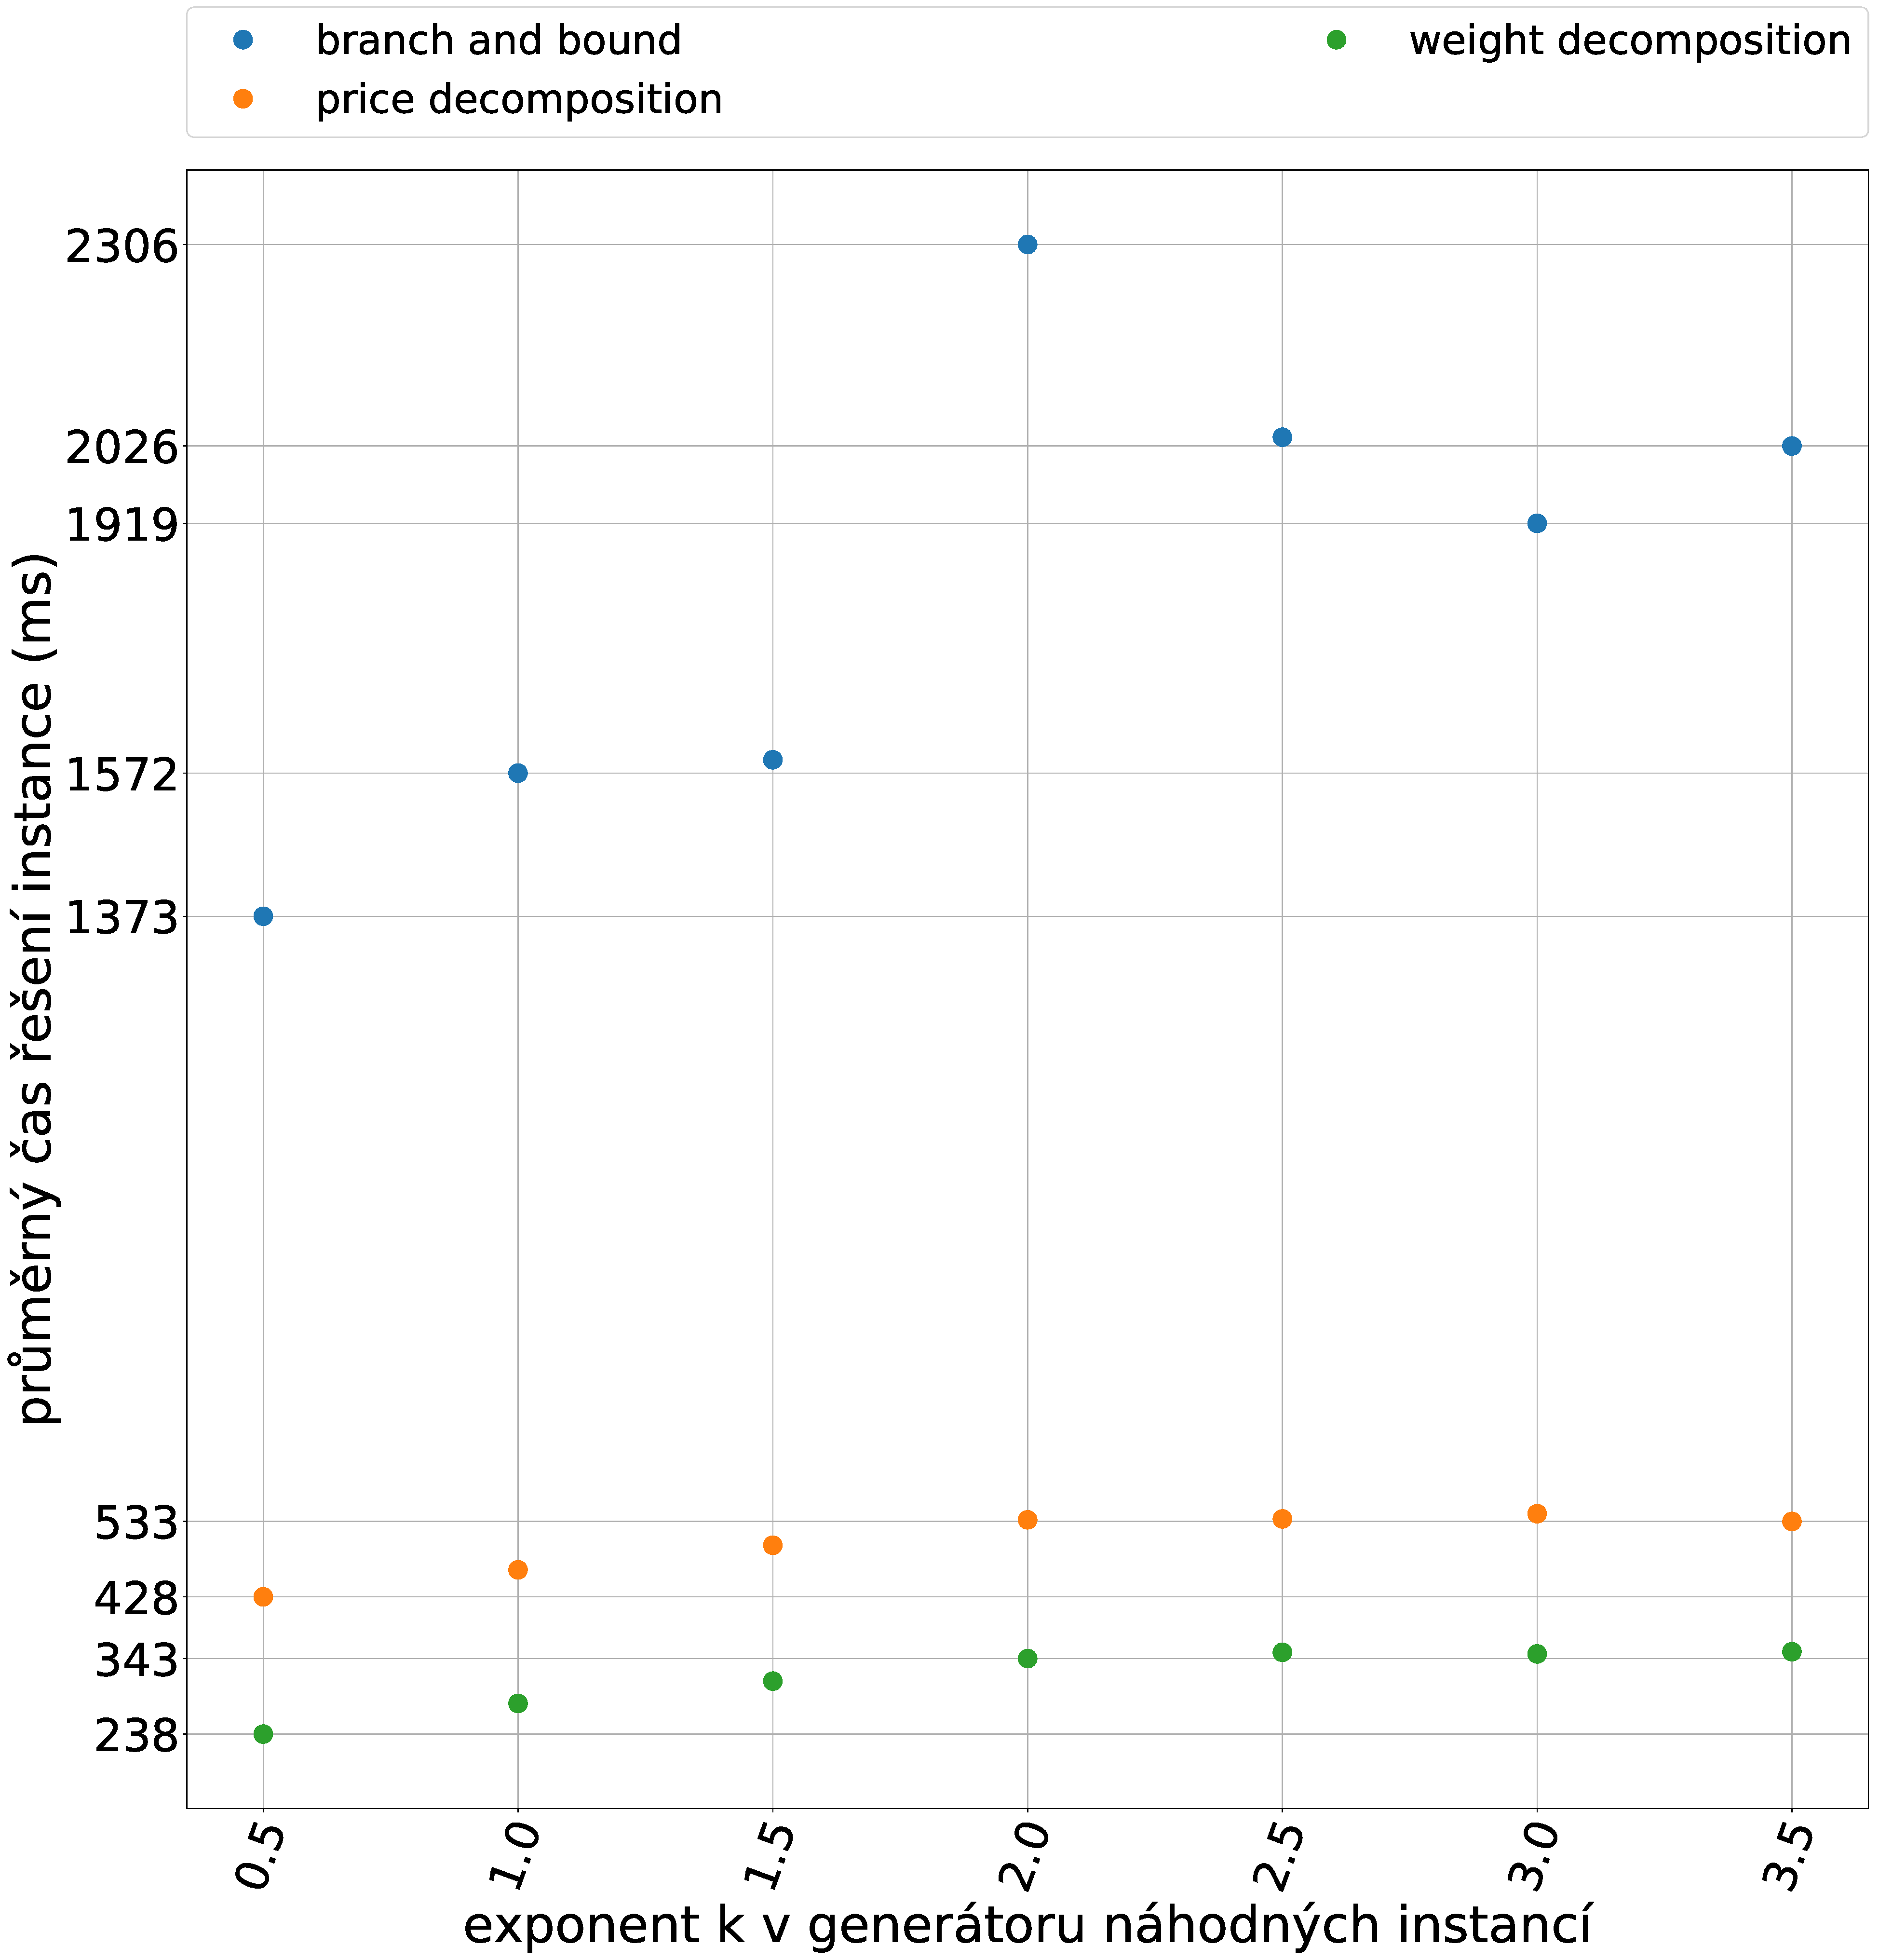
\includegraphics[width=\textwidth]{img/GVE.pdf} 
    \end{minipage}
    \begin{minipage}[c]{0.49\textwidth}
        \centering 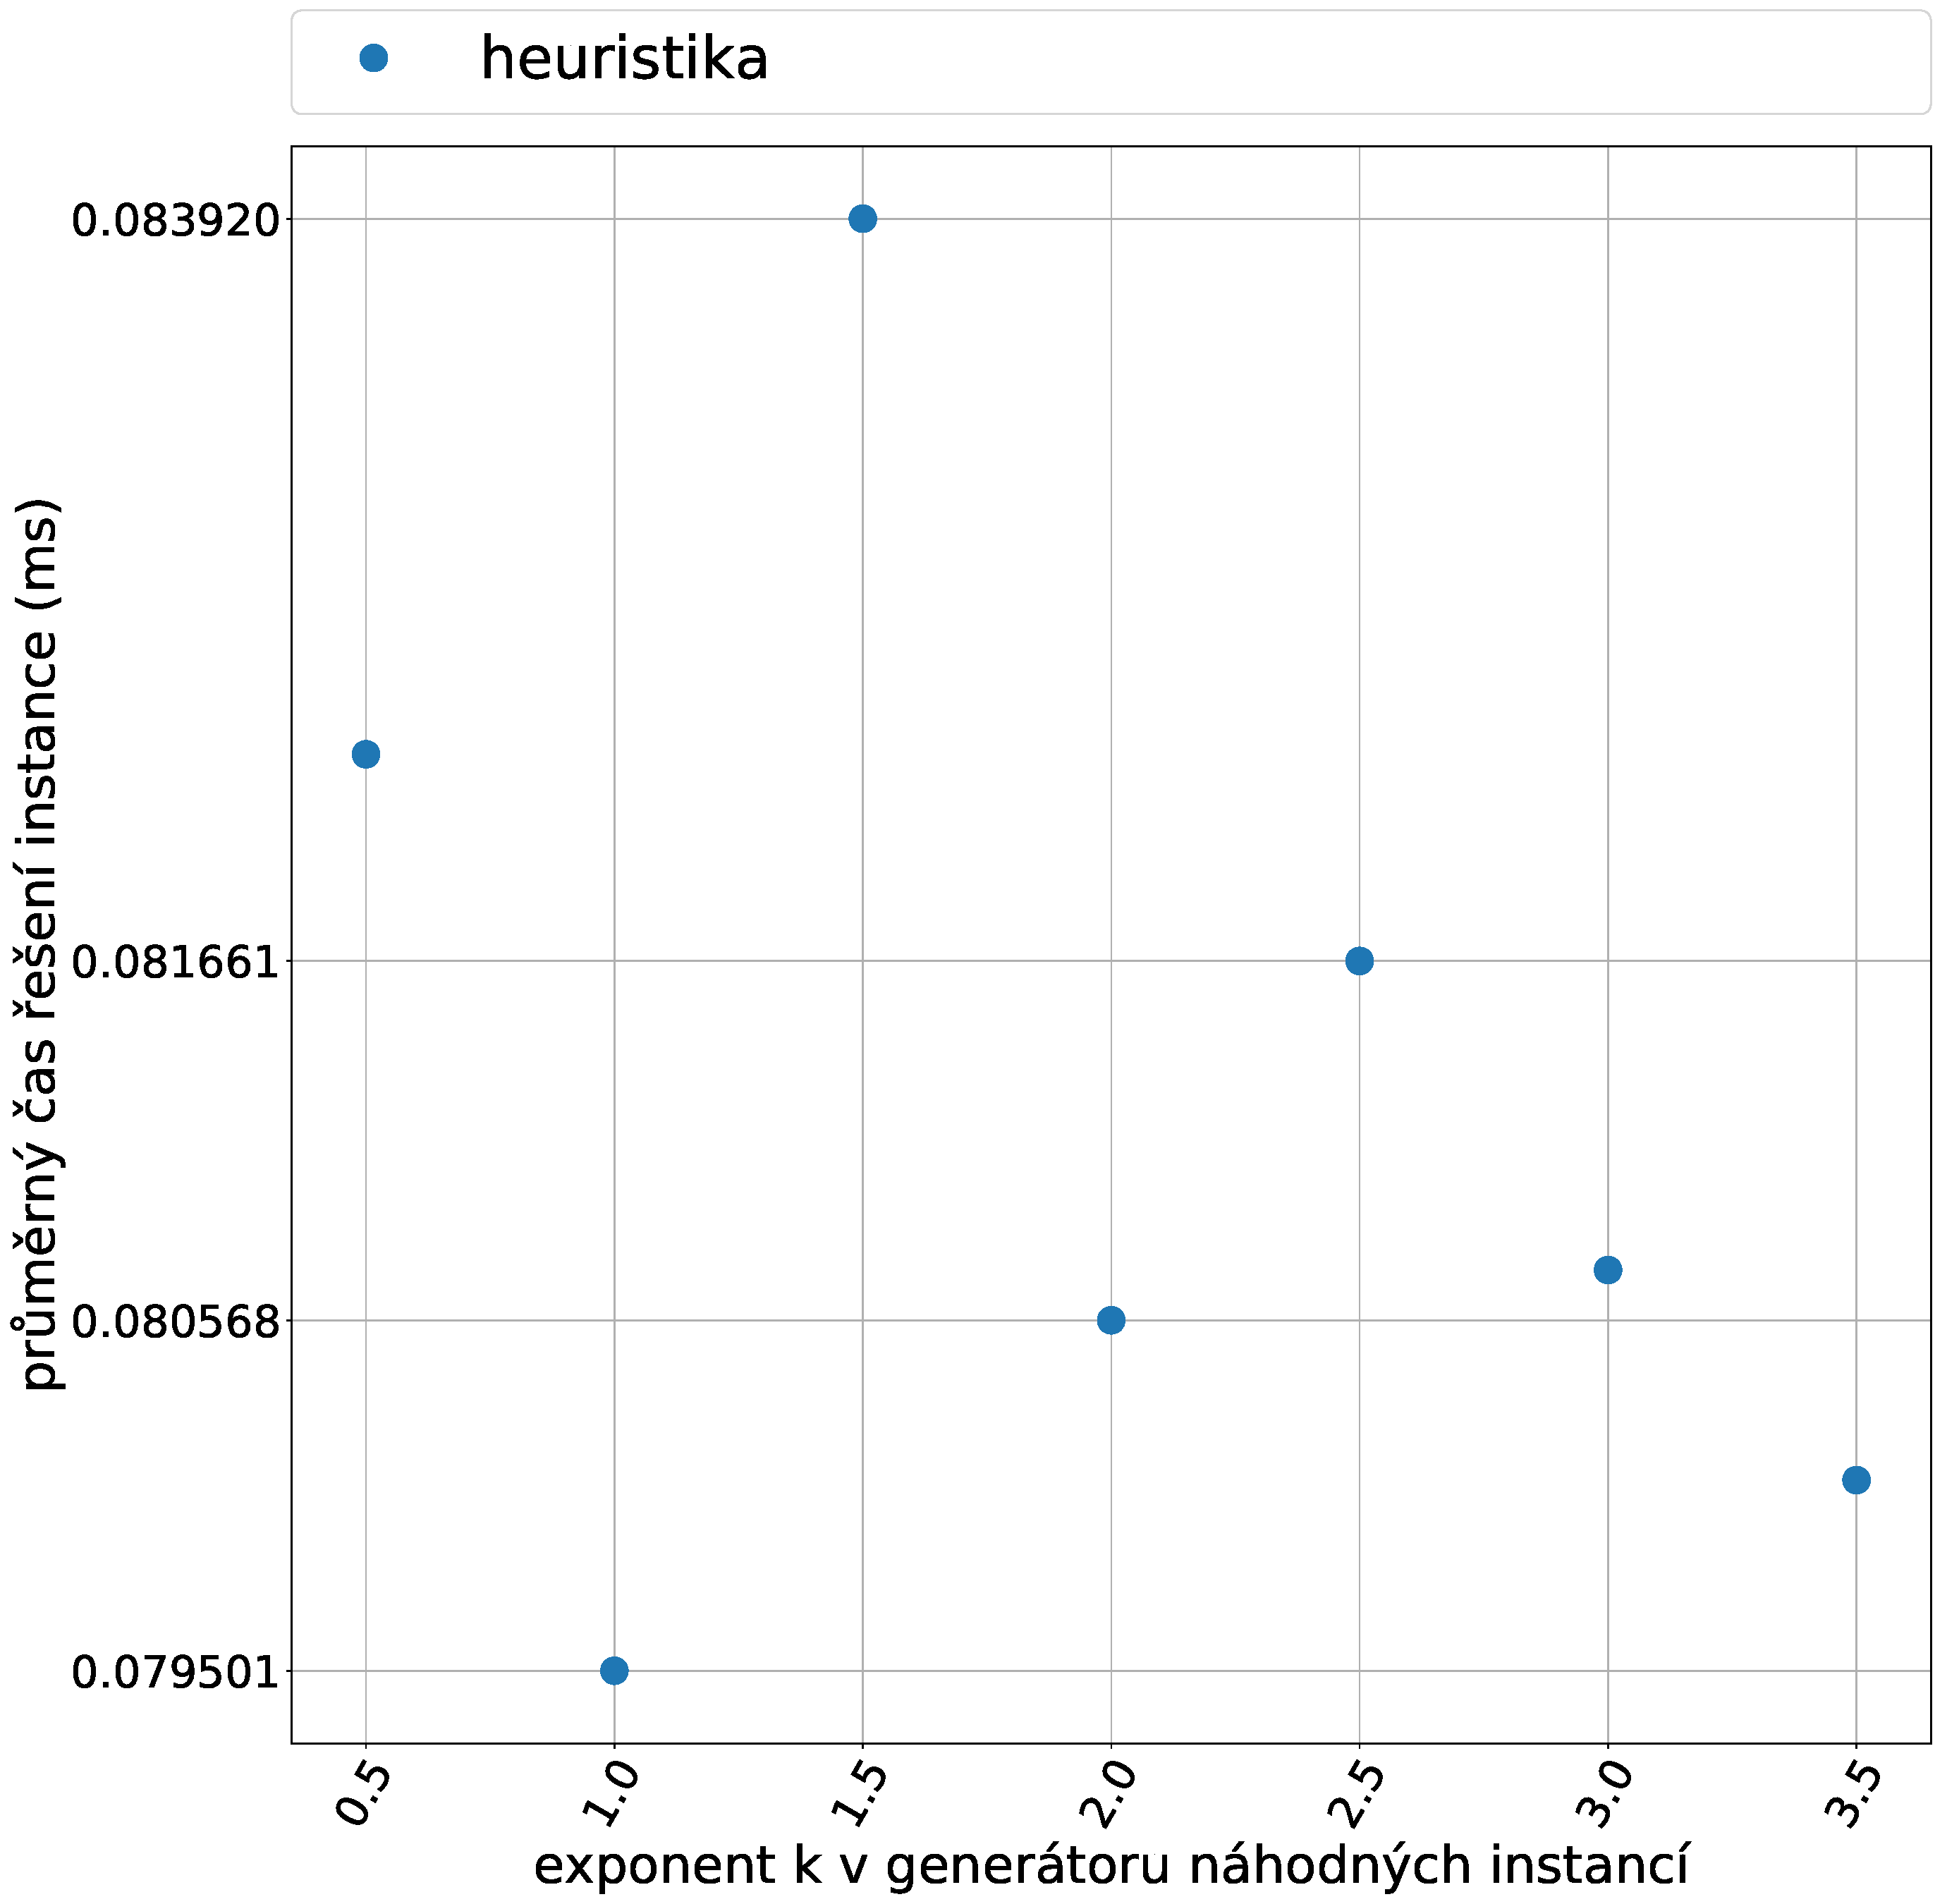
\includegraphics[width=\textwidth]{img/GVH.pdf} 
    \end{minipage}
    \\
   \caption{Na grafech je zobrazena časová náročnost jednotlivých medod v závislosti na granularitě instance. Zde jsou uvedeny grafy pro převahu velkých instancí, kde k je exponent z generátoru náhodných instancích, který určuje pravděpodobnost přijetí daného předmětu.}\label{fig:GVI}
    \end{figure} 
    
    \begin{figure}
	\centering
    \begin{minipage}[c]{0.49\textwidth}
        \centering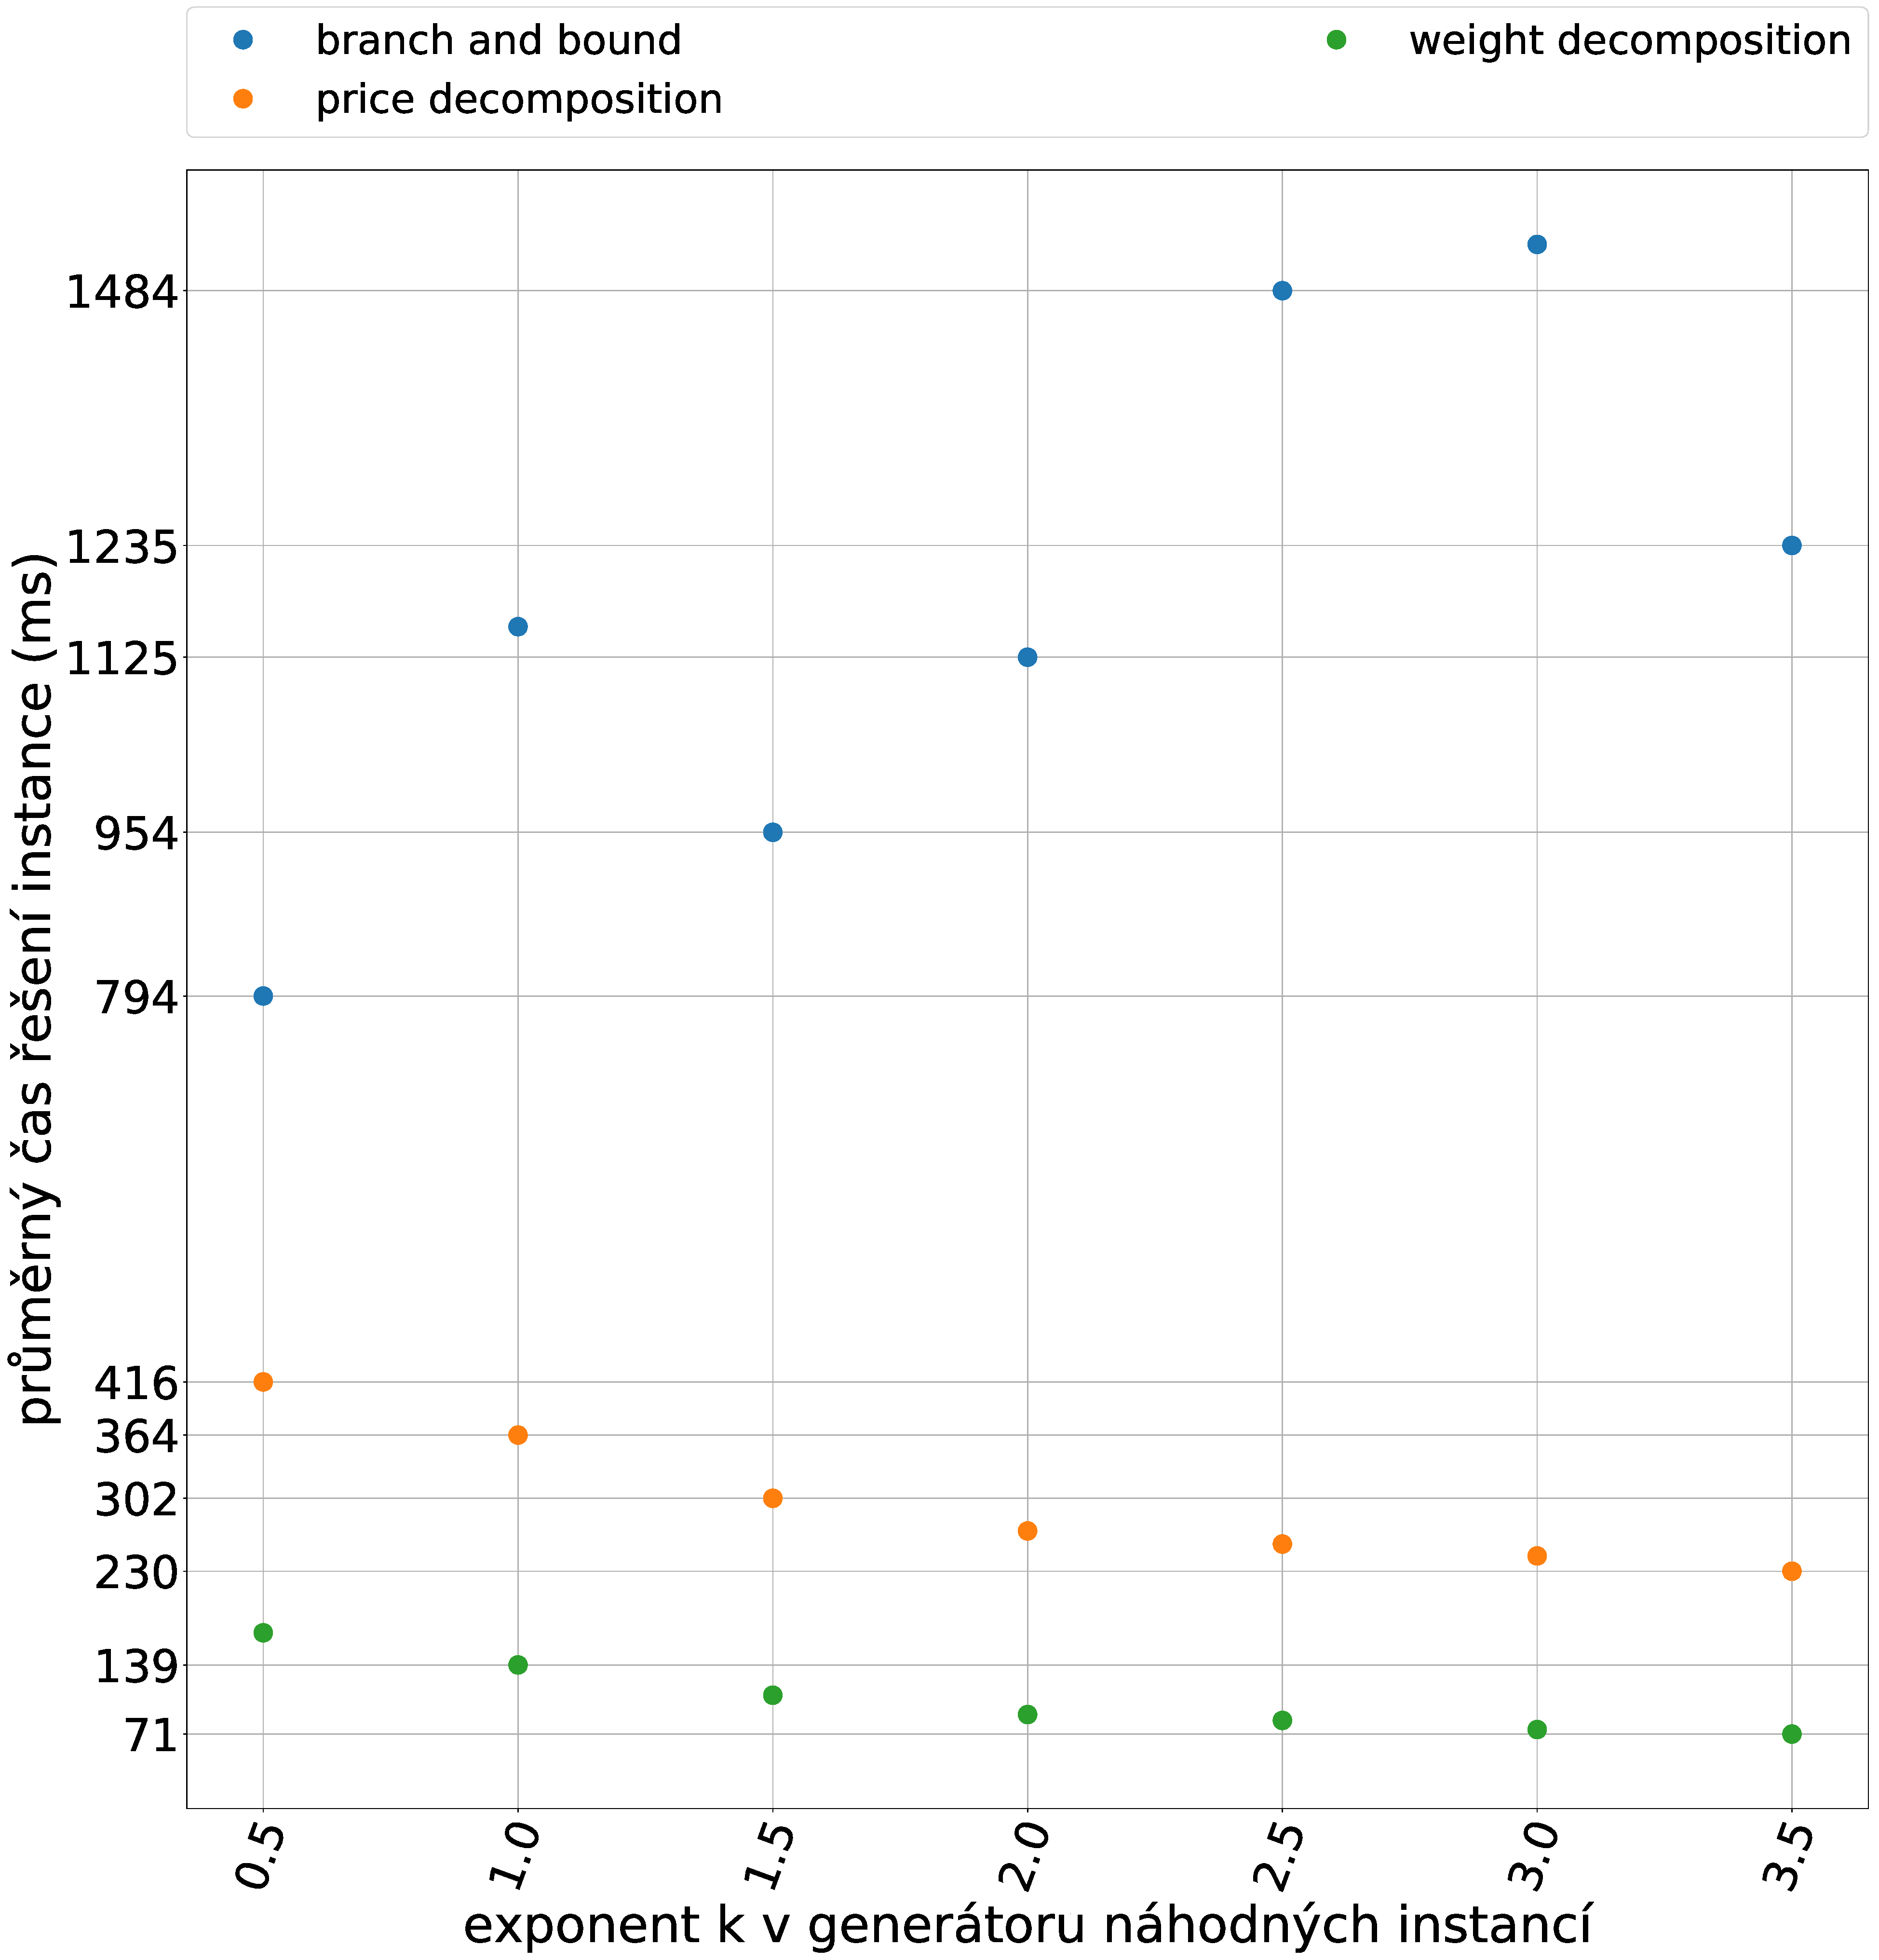
\includegraphics[width=\textwidth]{img/GME.pdf} 
    \end{minipage}
    \begin{minipage}[c]{0.49\textwidth}
        \centering 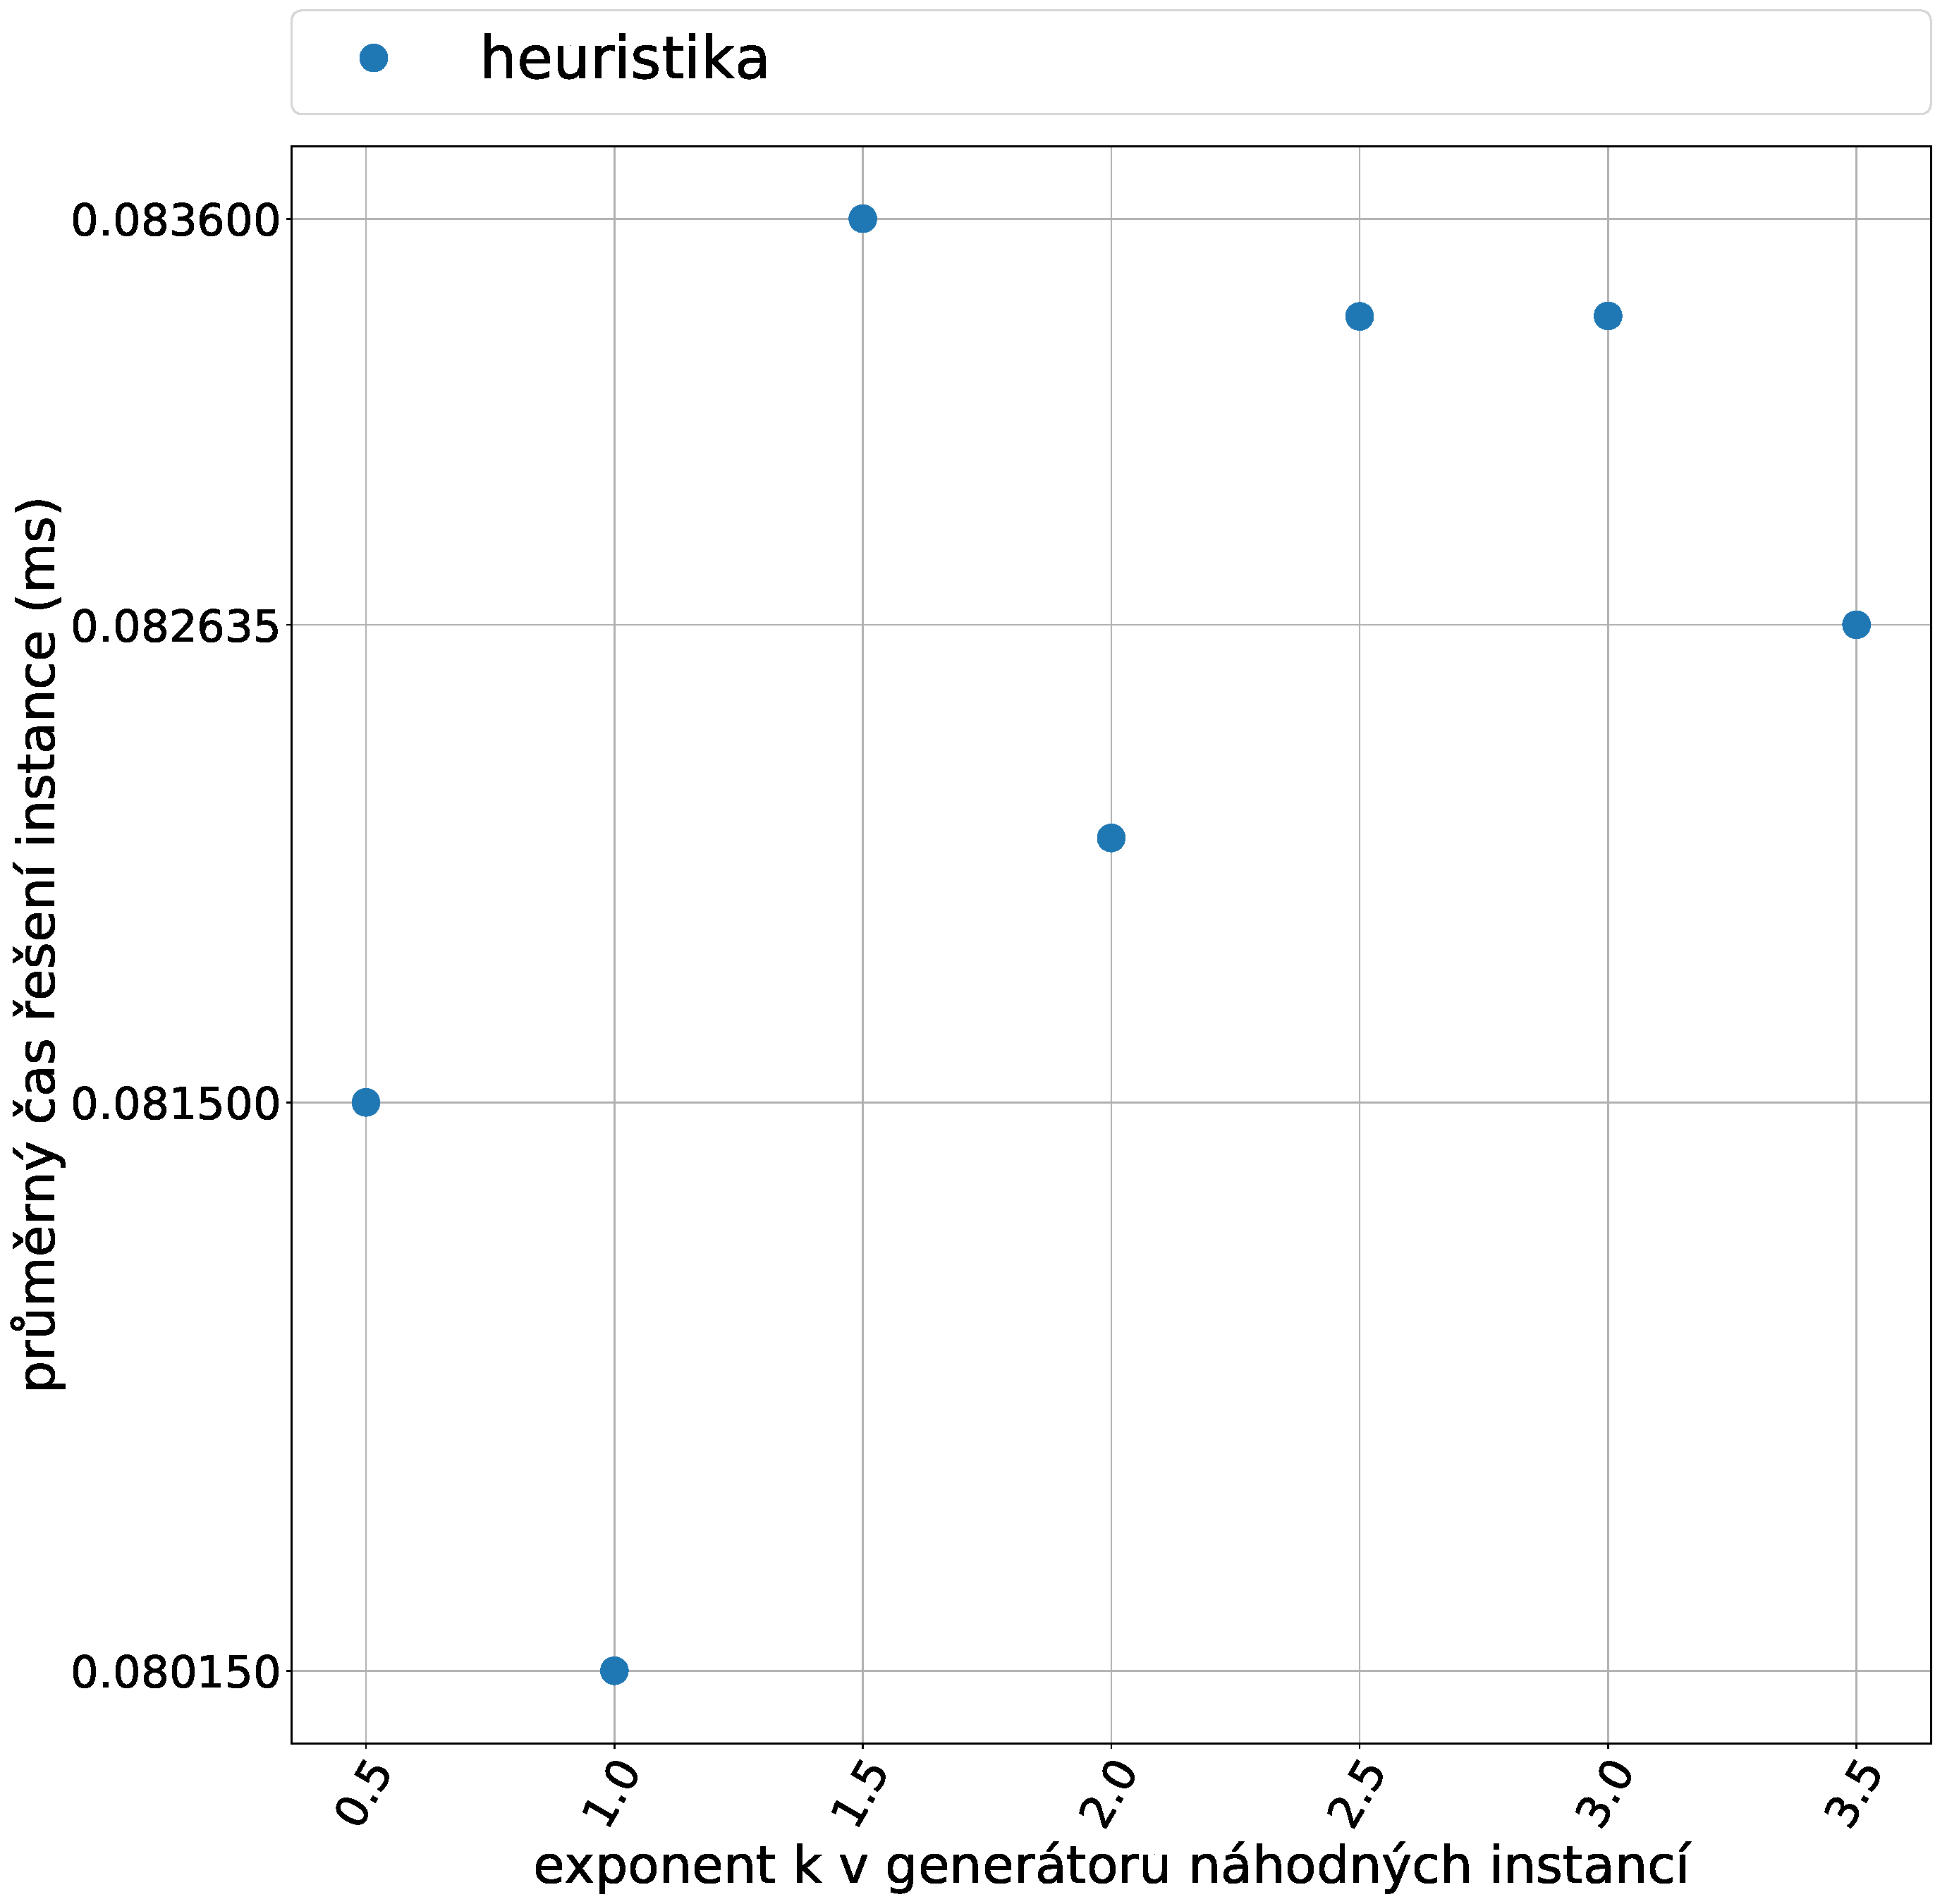
\includegraphics[width=\textwidth]{img/GMH.pdf} 
    \end{minipage}
    \\
   \caption{Na grafech je zobrazena časová náročnost jednotlivých medod v závislosti na granularitě instance. Zde jsou uvedeny grafy pro převahu malých instancí, kde k je exponent z generátoru náhodných instancích, který určuje pravděpodobnost přijetí daného předmětu.}\label{fig:GMI}
    \end{figure} 
 

 
 
Experimenty jsem prováděl v režimu jednoho vlákna na starším datovém serveru v podobě starého notebooku, který v době výpočtu nebyl používán. Výsledky tedy nejsou ovlivněny jinými běžícími programy. Procesor na testovacím stroji: \textit{Intel Pentium T3400 (2 cores). Taktován na 2.16~GHz s~1~MB cache}.
Měření času CPU probíhalo v knihovně $timeit$ s tidíci násobným průchodem pro jednotlivá měření pro přesnost měření.

Pro každý parametr bylo vygenerováno 100 instancí o počtu předmětů 27. Na grafech jsem vždy rozdělil exaktní metody a heuristiku z důvodu nízkých časů u heuristiky, u které by nebyly rozdíly s exaktními metodami vůbec ukázatelné. 


\subsection{Závislost na granularitě instance}
První jsem se podíval na granularitu instancí. Ta je řízena následovně. V generátoru je možno ovlivnit, zda instance bude obsahovat spíše malé nebo spíše velké věci. Pro převahu malých věcí je pravděpodobnost $p$, že věc s váhou $w$ bude v instanci zahrnuta $$ p=\frac{1 }{ w^k}$$. Kde $k$ je volitelný exponent. Pro převahu velkých věcí platí symetrický vztah $$ p=\frac{1}  {(w_{max}-w)^k}$$.

Na grafu \ref{fig:GVI} můžeme vidět porovnání pro převahu velkých věcí. Lze vidět, že pro metody větví a hranic je zde jasně patrný trend. S větším počtem velkých předmětů tedy roste její výpočetní náročnost. Tento trend, avšak ne tak patný, může být pozorován i na jednotlivých dekompozicích. 

Na grafu \ref{fig:GMI} vidíme porovnání pro převahu malých věcí. I zde jsou patrné citlivosti jednotlivých exaktních metod. Ale mírně odlišně než u převahy velkých věcí. U metody větví a hranic je stále s převahou menších instancí roste její časová náročnost. Naopak u dekompozicích tento čas klesá. 

Citlivost u dekompozic bych si také mohl vysvětlit jako citlivost na celkovou sumu váhy nebo ceny podle druhu dekompozice. Protože převaha velkých nebo malých předmětů tuto sumu ovlivní. Citlivost na tyto parametry prozkoumáme v další podkapitole.

U heuristické metody na grafech můžeme fidět veliký rozptyl hodnot. Její závislost na granularitě se tady nepotvrdila. O této metodě bych tedy neřekl, že její výkonost ovlivní granularita jednotlivých instancí.

Na grafech \ref{fig:GOEI} je ukázána průměrná a maximální chyba heuristické metody při změnách granularity instancí. Zde není patrná témě žádná závislost chyby na granularitě instance. Při podrobnější zkoumální hodnot maxim, by možná bylo možné říct, že maximální chyba klesá s převahou malých i velkých předmětů, ale tento trend by bylo nutné podrobněji prozkoumat a podrobit mnohem větší analýze.
 
 \begin{figure}
	\centering
    \begin{minipage}[c]{0.49\textwidth}
        \centering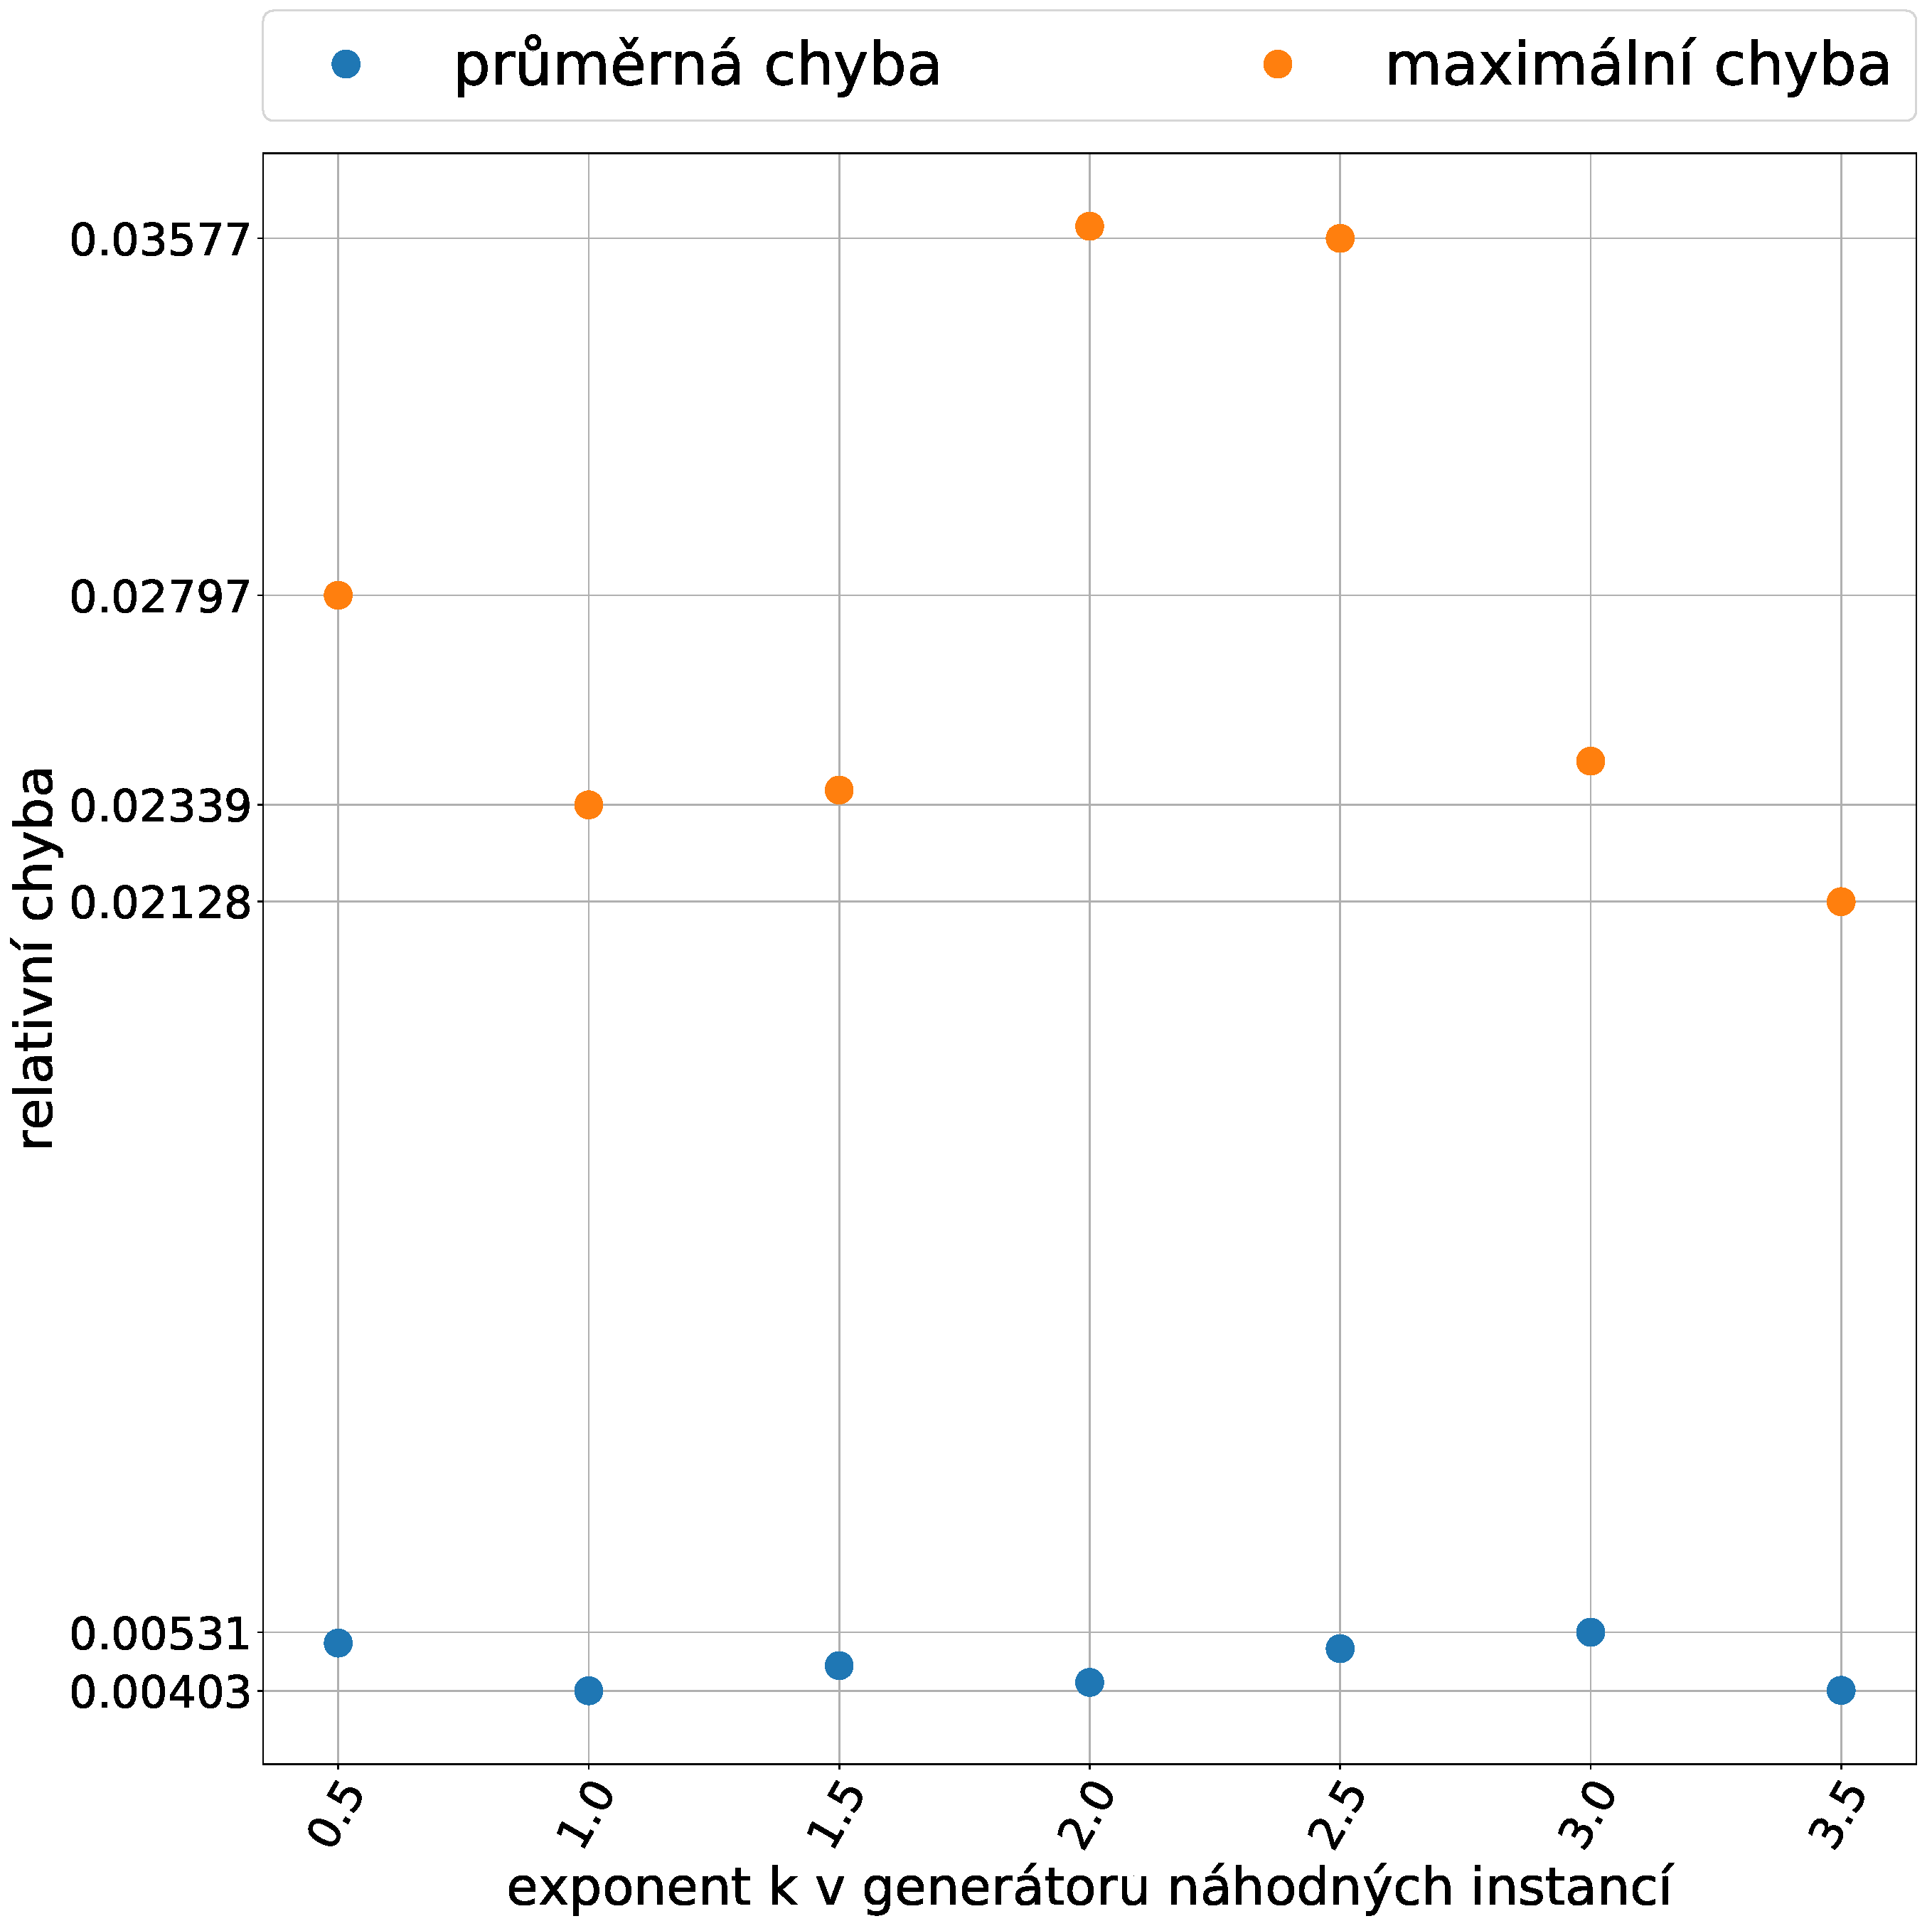
\includegraphics[width=\textwidth]{img/GMHE.pdf} 
    \end{minipage}
    \begin{minipage}[c]{0.49\textwidth}
        \centering 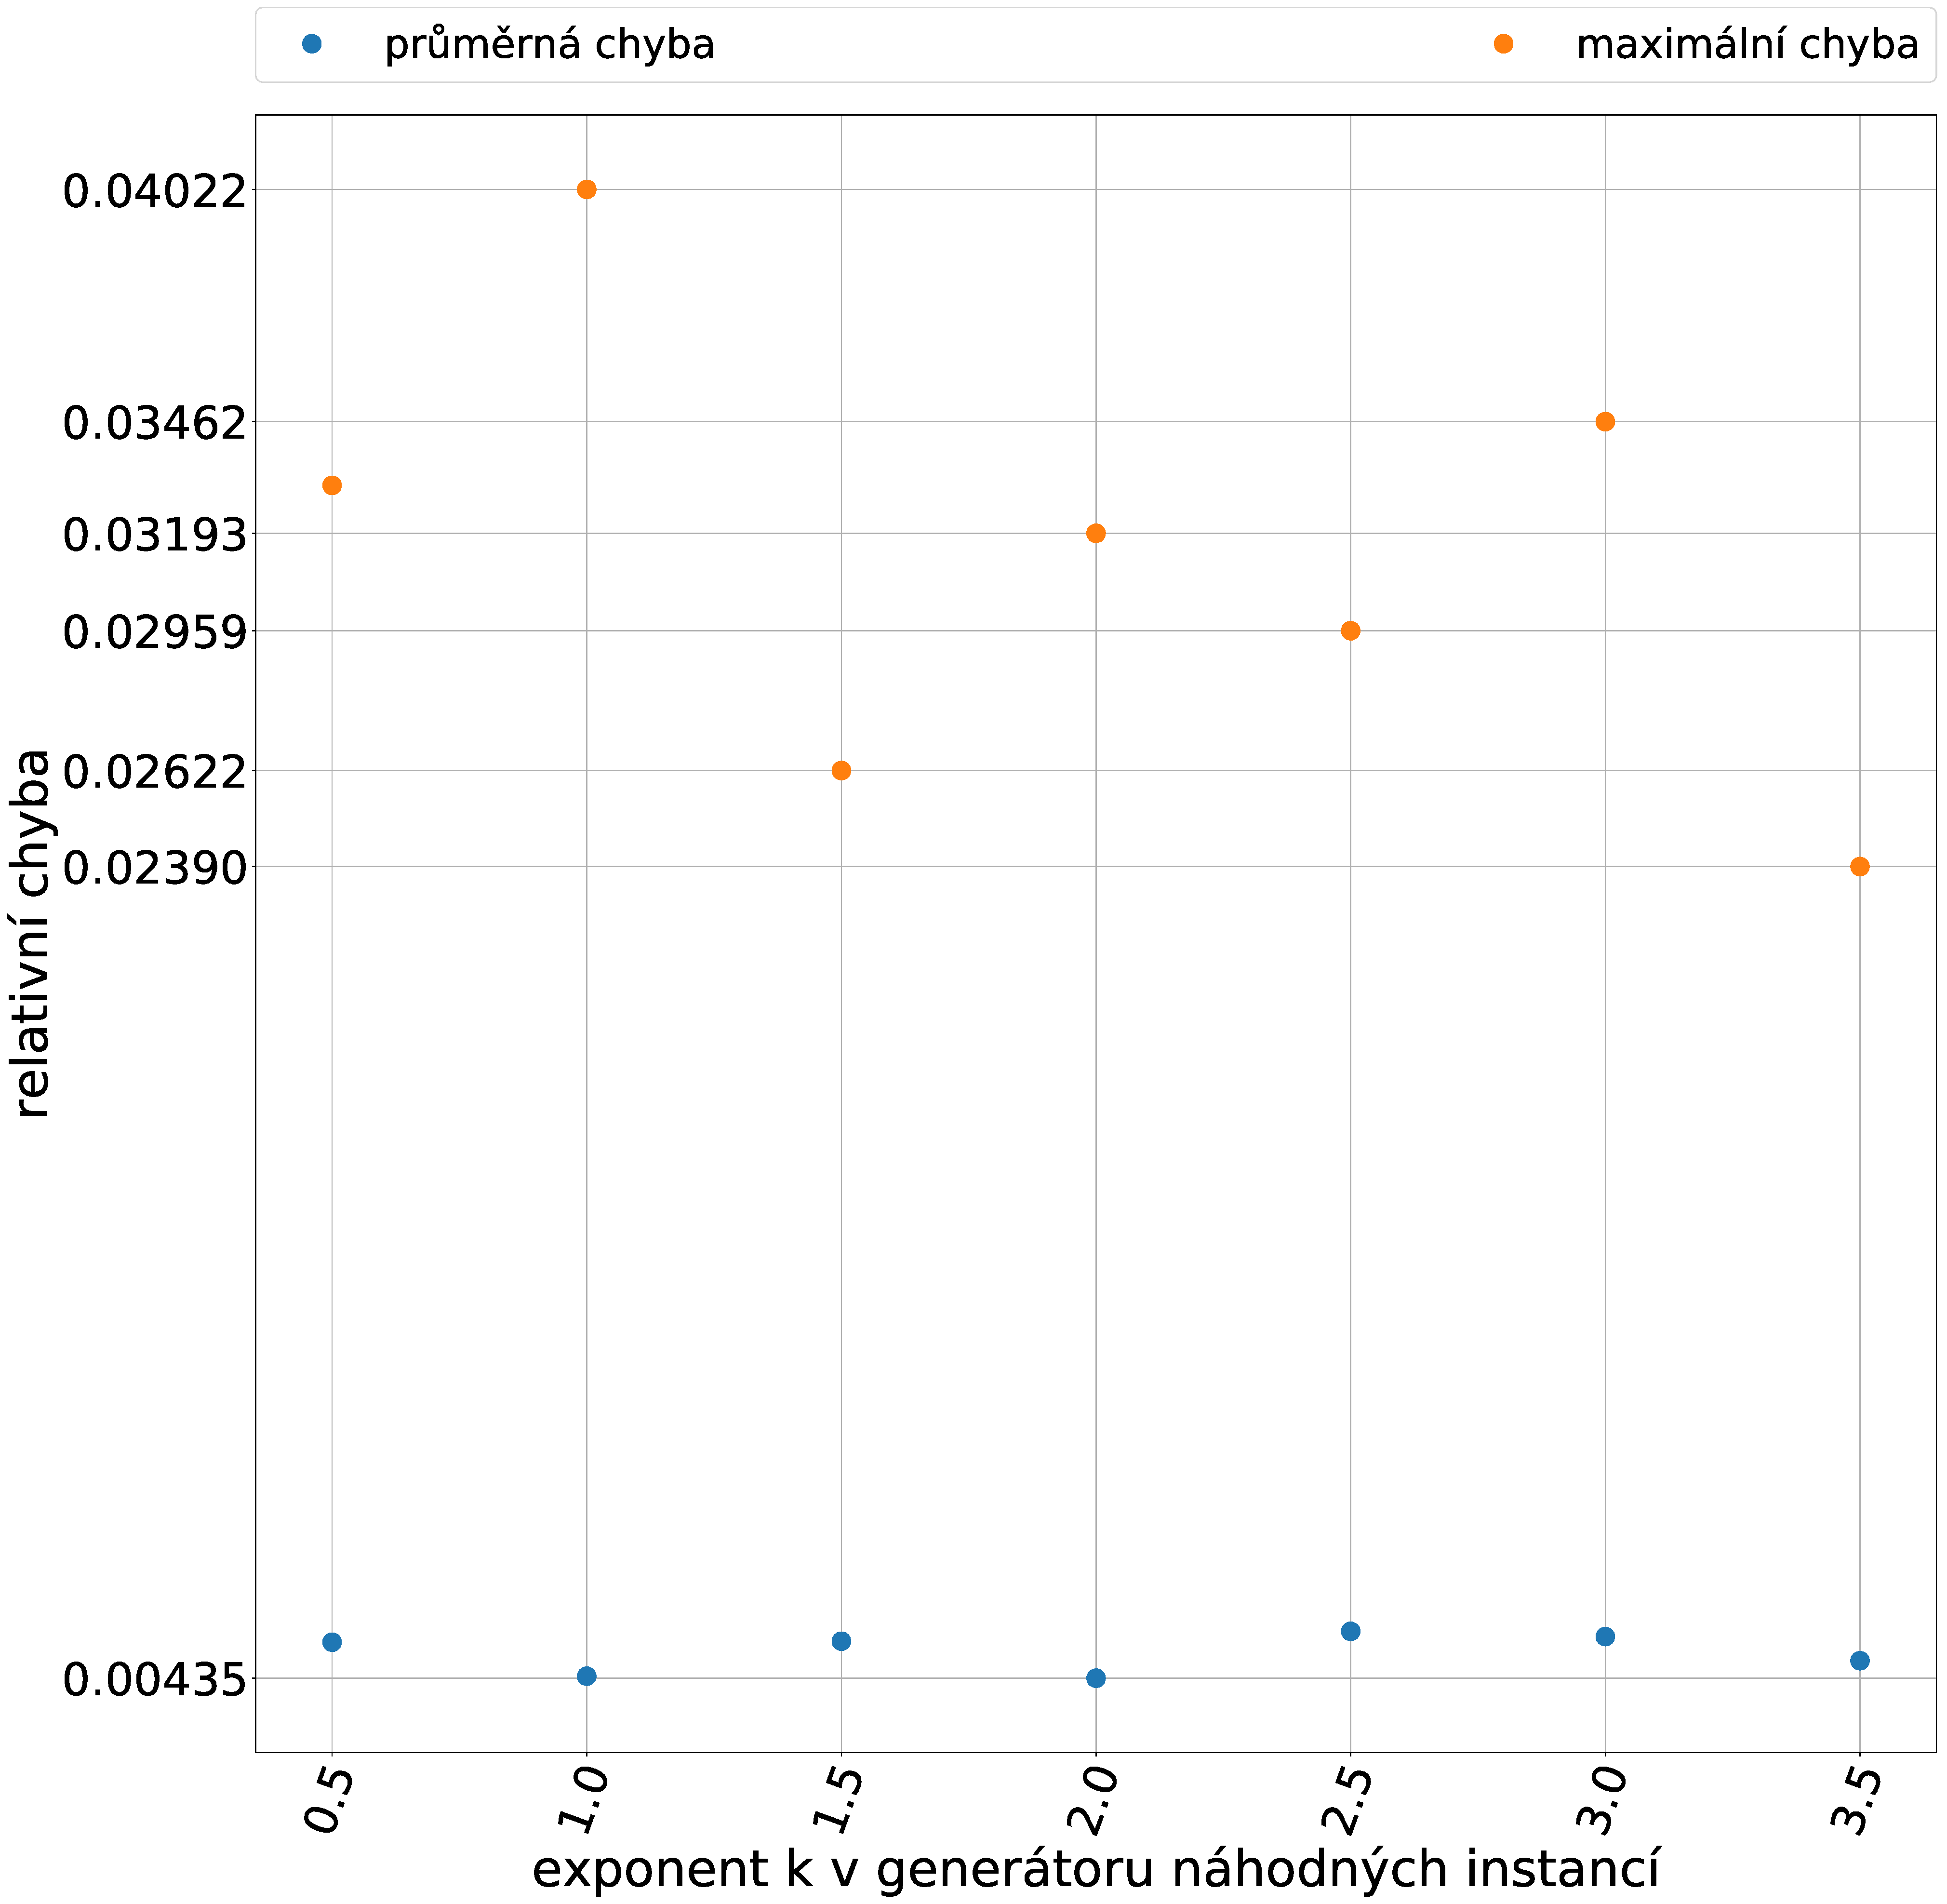
\includegraphics[width=\textwidth]{img/GVHE.pdf} 
    \end{minipage}
    \\
   \caption{Na grafech je ukázána vždy průměrná a maximální chyba heuristiky v závislosti na granularitě instance. Na levém grafu pro převahu malých instancí a na převém grafu pro převahu velkých instancí.}\label{fig:GOEI}
    \end{figure} 
    
\subsection{Závislost na poměru součtu vah předmětů k nosnosti batohu}
\begin{figure}
	\centering
    \begin{minipage}[c]{0.49\textwidth}
        \centering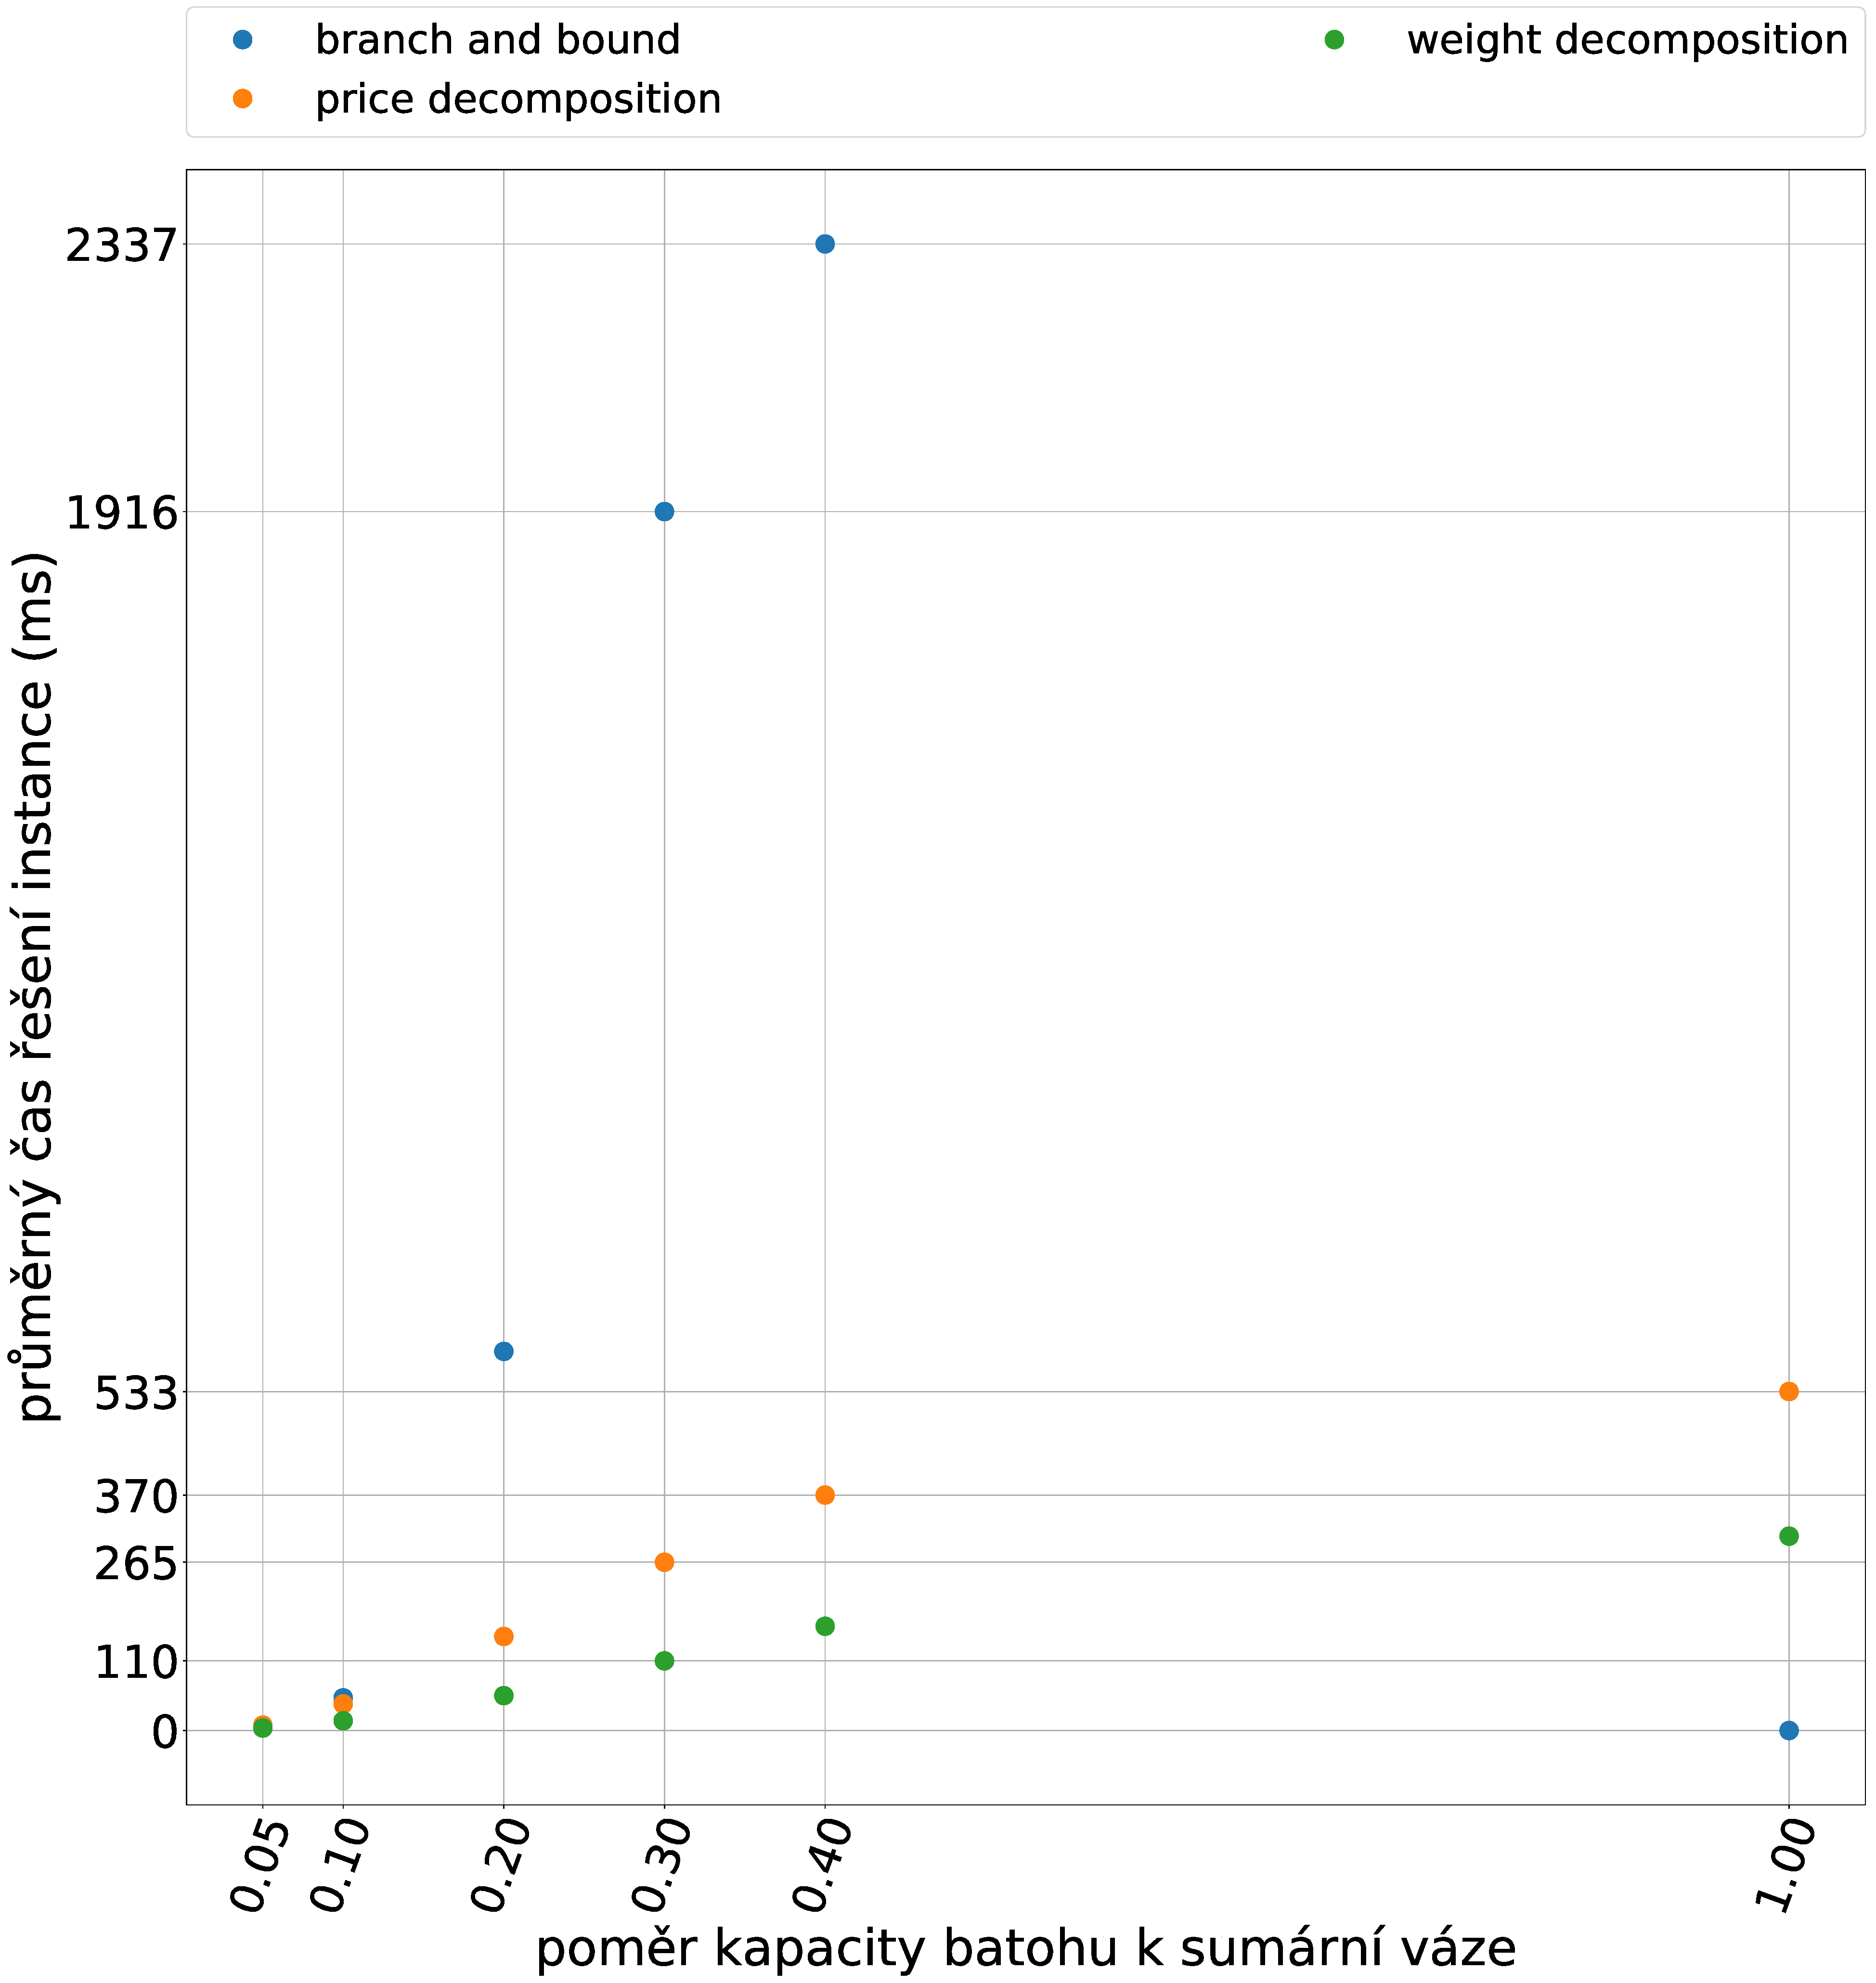
\includegraphics[width=\textwidth]{img/mE.pdf} 
    \end{minipage}
    \begin{minipage}[c]{0.49\textwidth}
        \centering 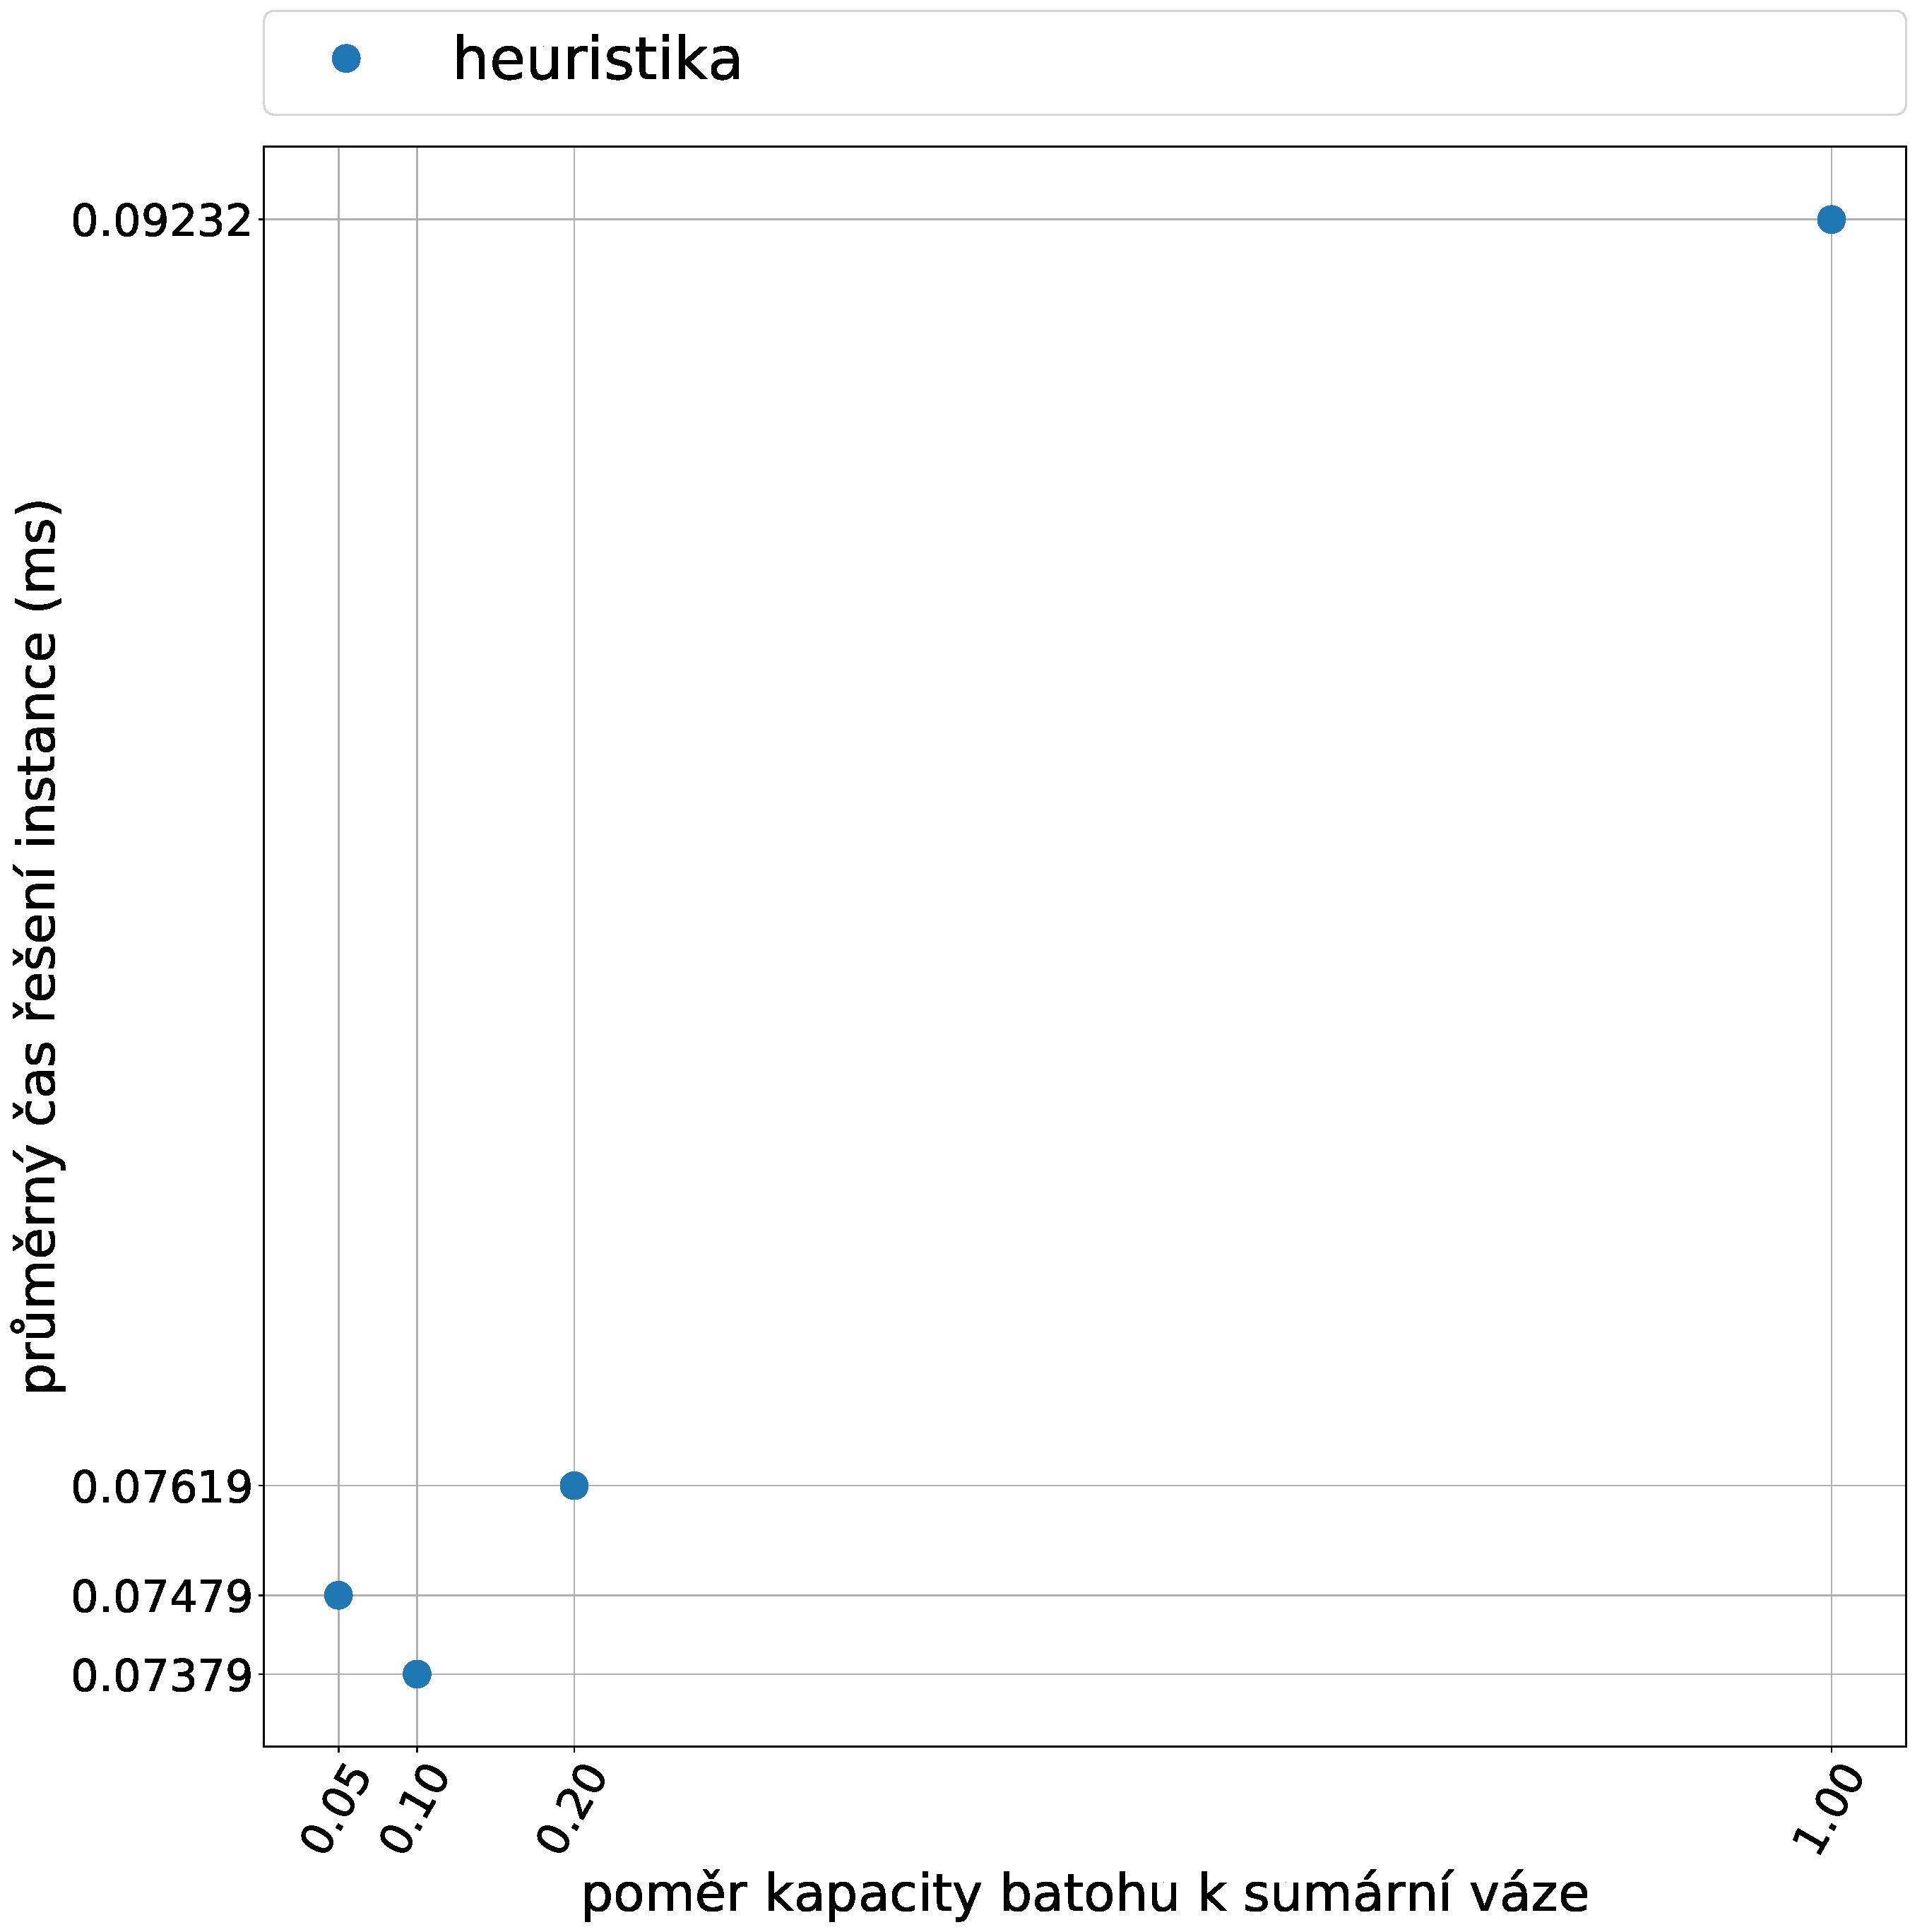
\includegraphics[width=\textwidth]{img/mH.pdf} 
    \end{minipage}
    \\
   \caption{Na grafech je ukázána vždy průměrná a maximální chyba heuristiky v závislosti na granularitě instance. Na levém grafu pro převahu malých instancí a na převém grafu pro převahu velkých instancí.}\label{fig:GOEI}
    \end{figure} 
    
    

\begin{figure}[h]\centering
	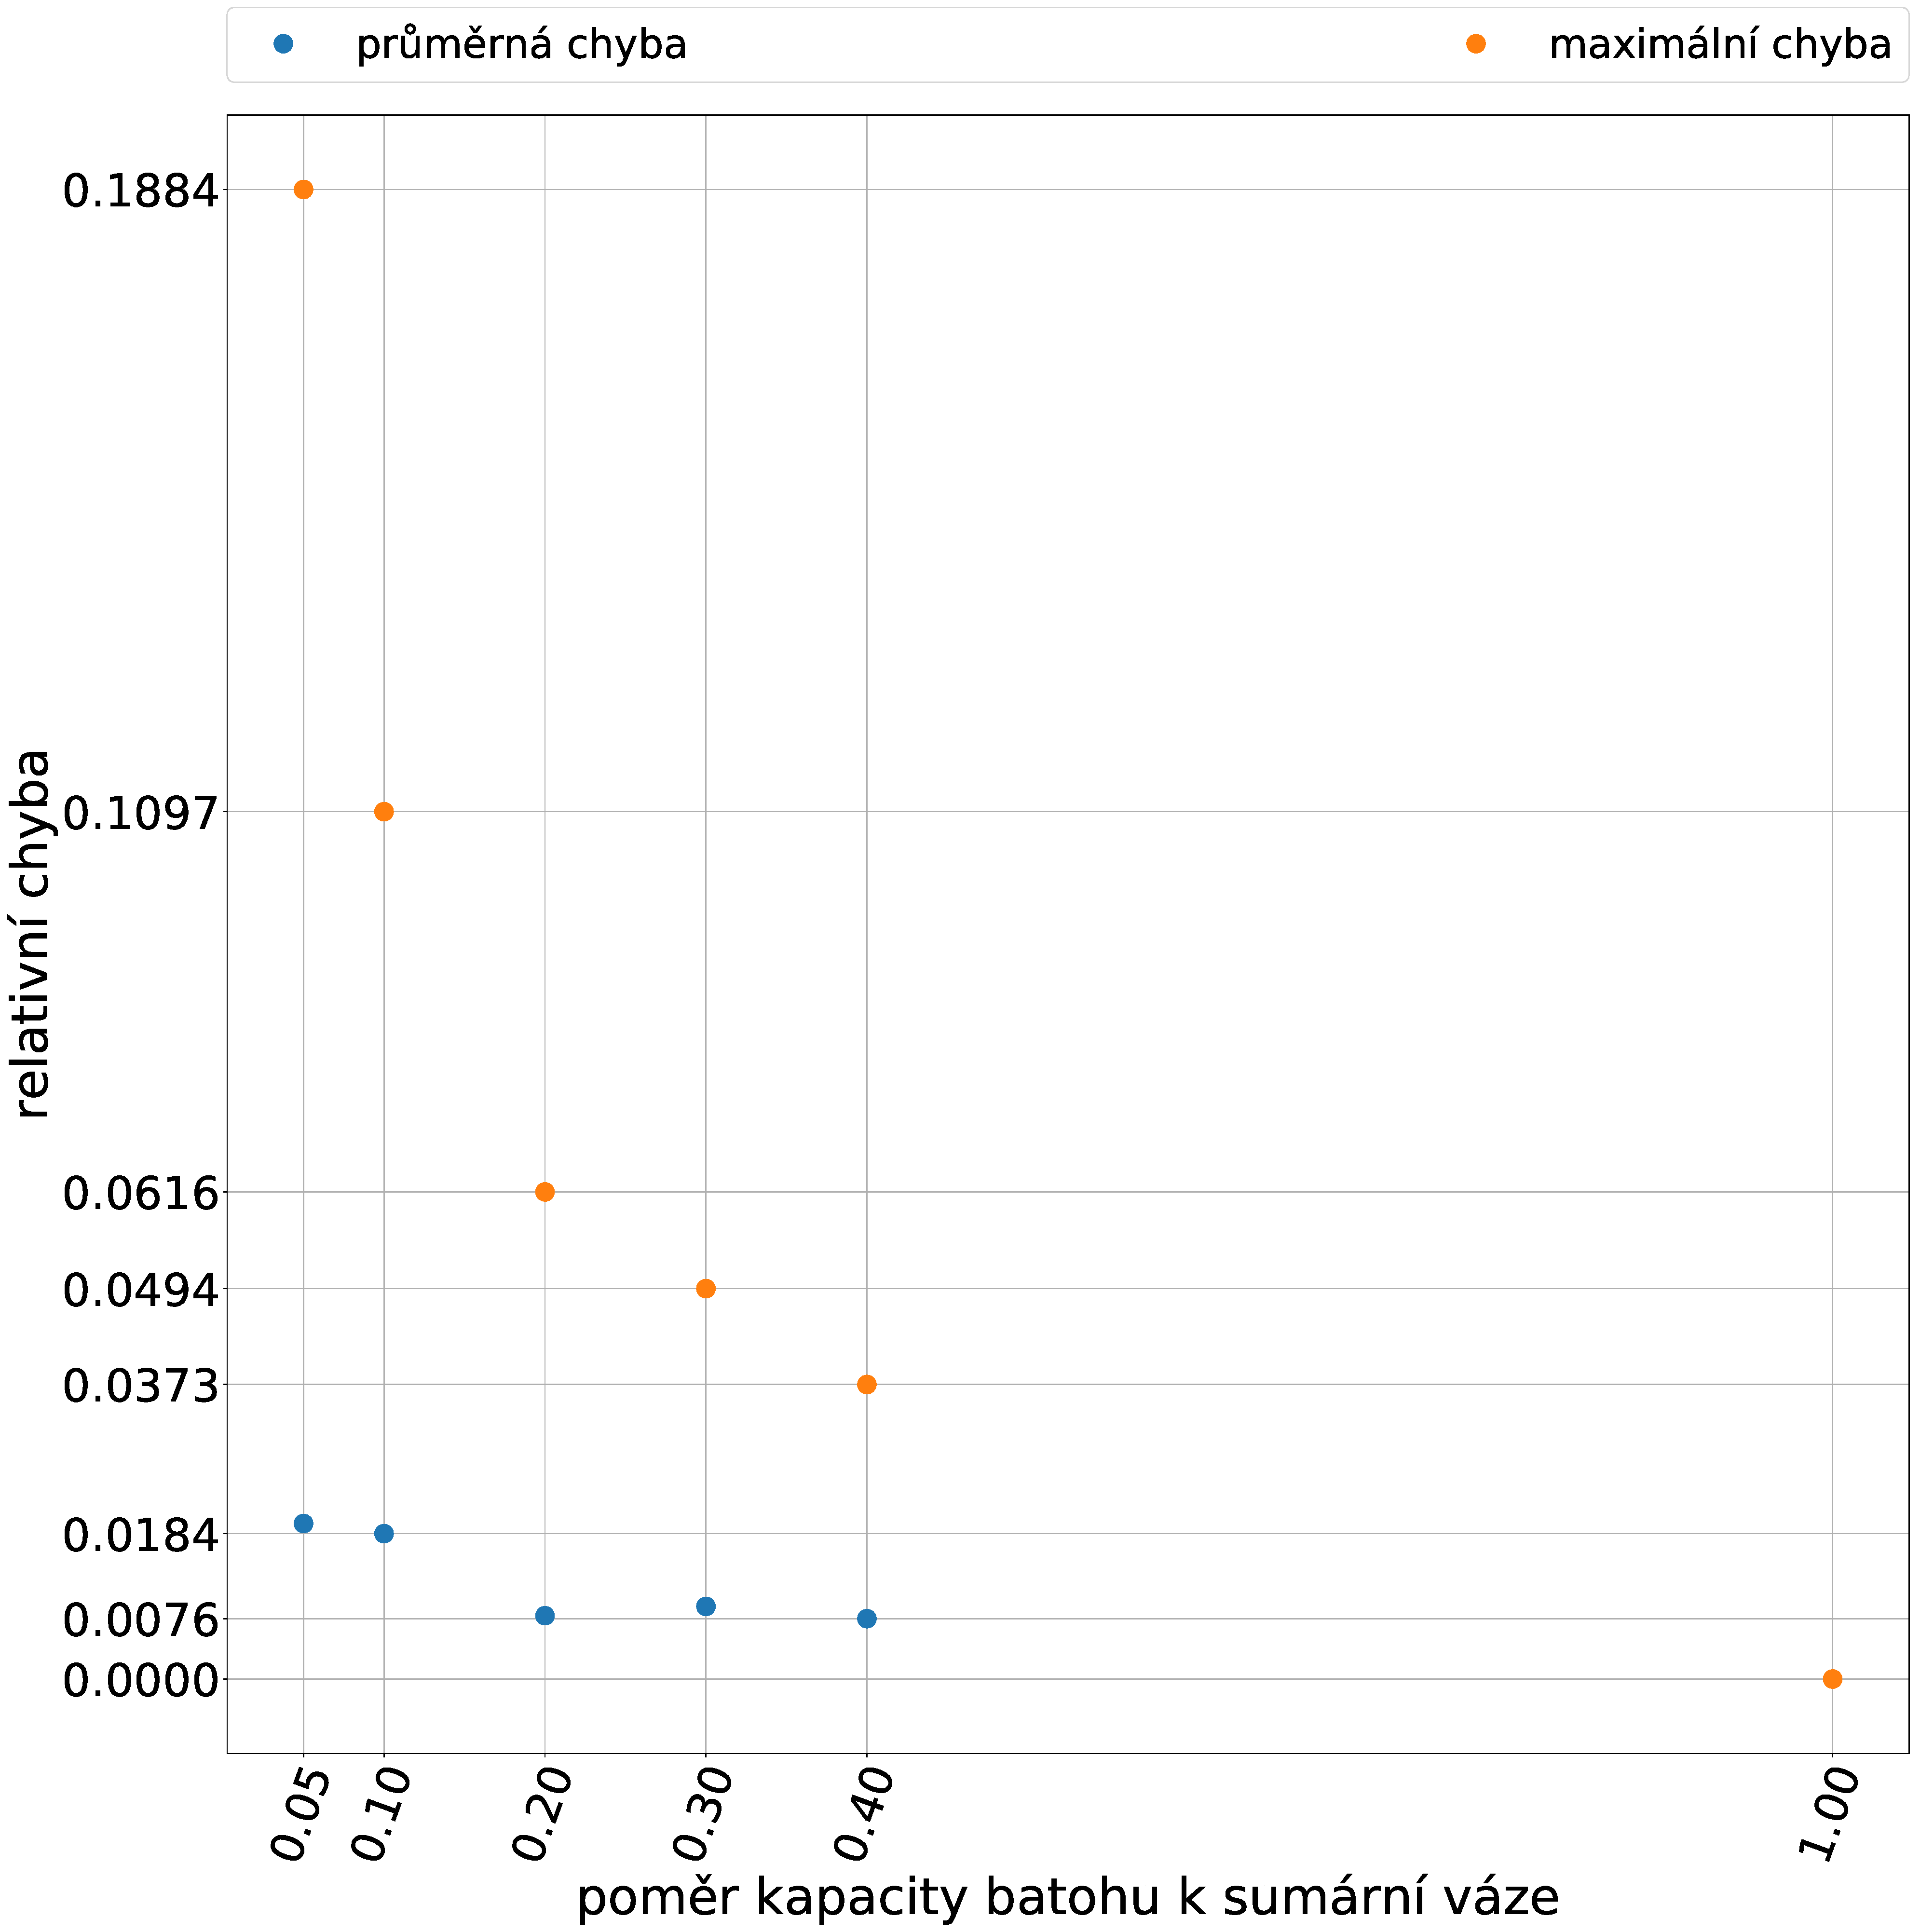
\includegraphics[scale=0.2]{img/mHE}
 	\caption[1]{Brute-force ve srovnání s dynamickým programováním s dekompozicí podle ceny. Časová náročnost. Na grafu jsou průměrné hodnoty.}\label{fig:1}
 \end{figure} 	

\subsection{Závislost na maximální ceně předmětů}

\begin{figure}
	\centering
    \begin{minipage}[c]{0.49\textwidth}
        \centering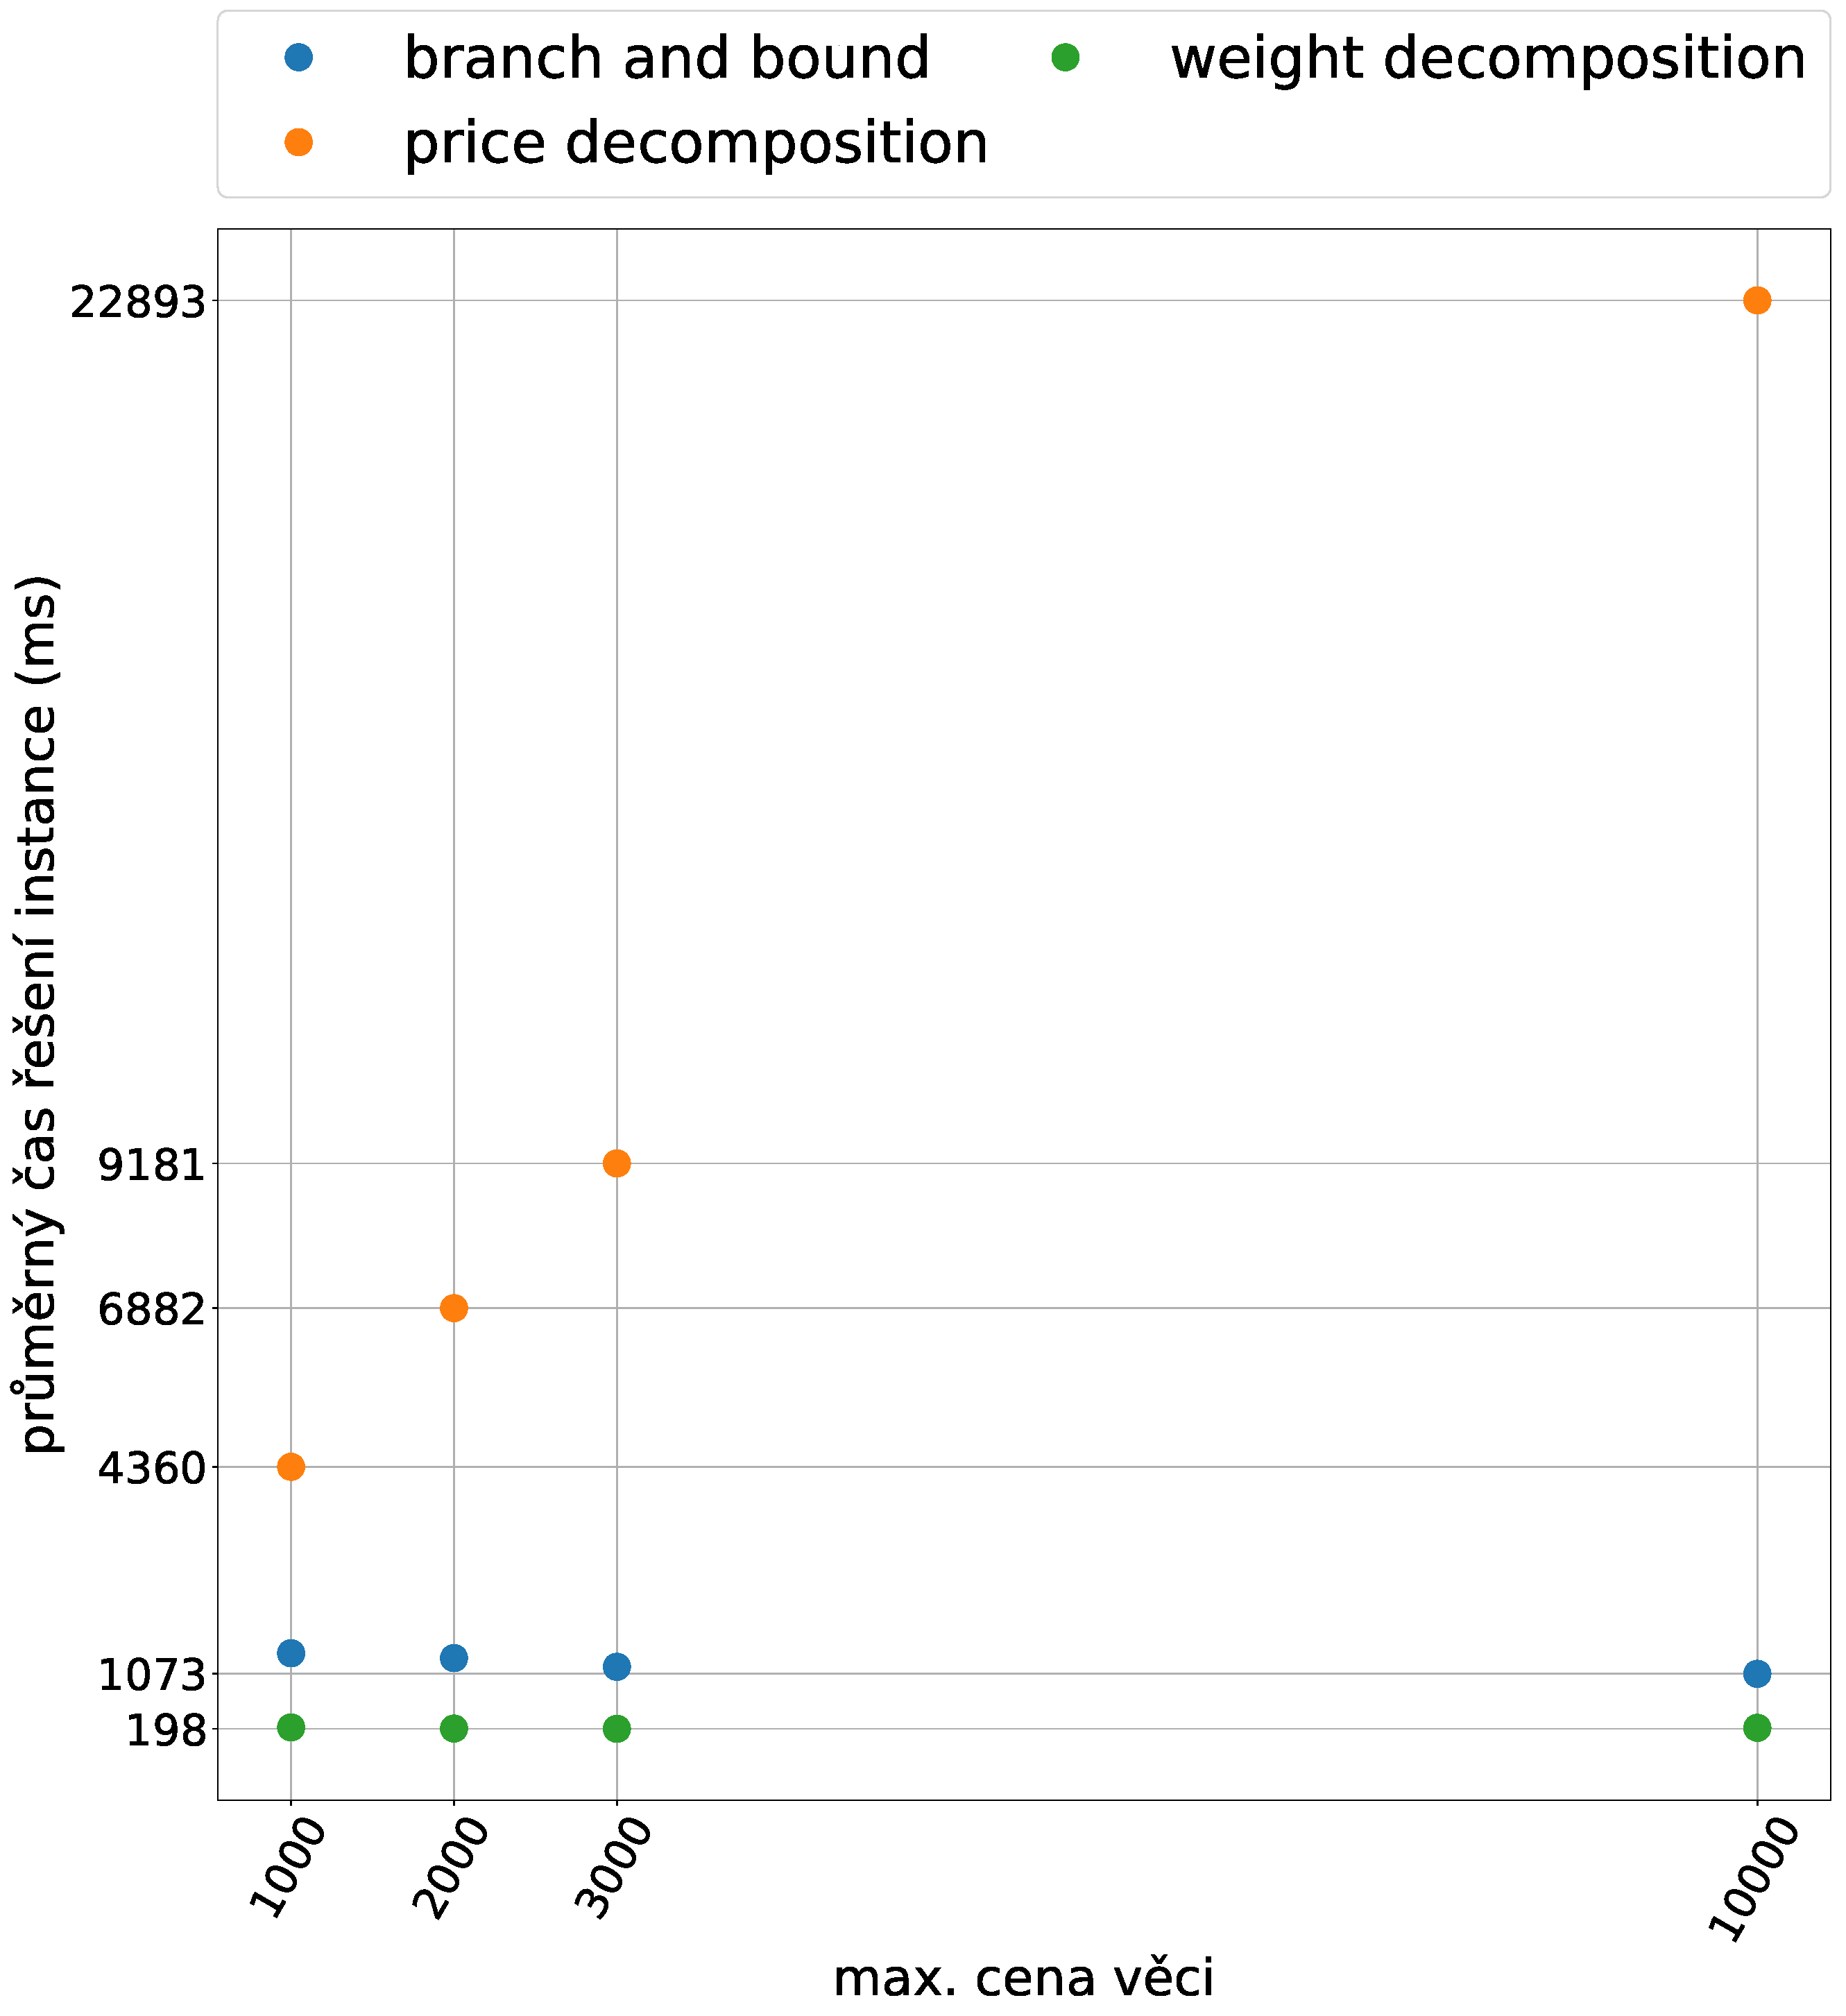
\includegraphics[width=\textwidth]{img/CE.pdf} 
    \end{minipage}
    \begin{minipage}[c]{0.49\textwidth}
        \centering 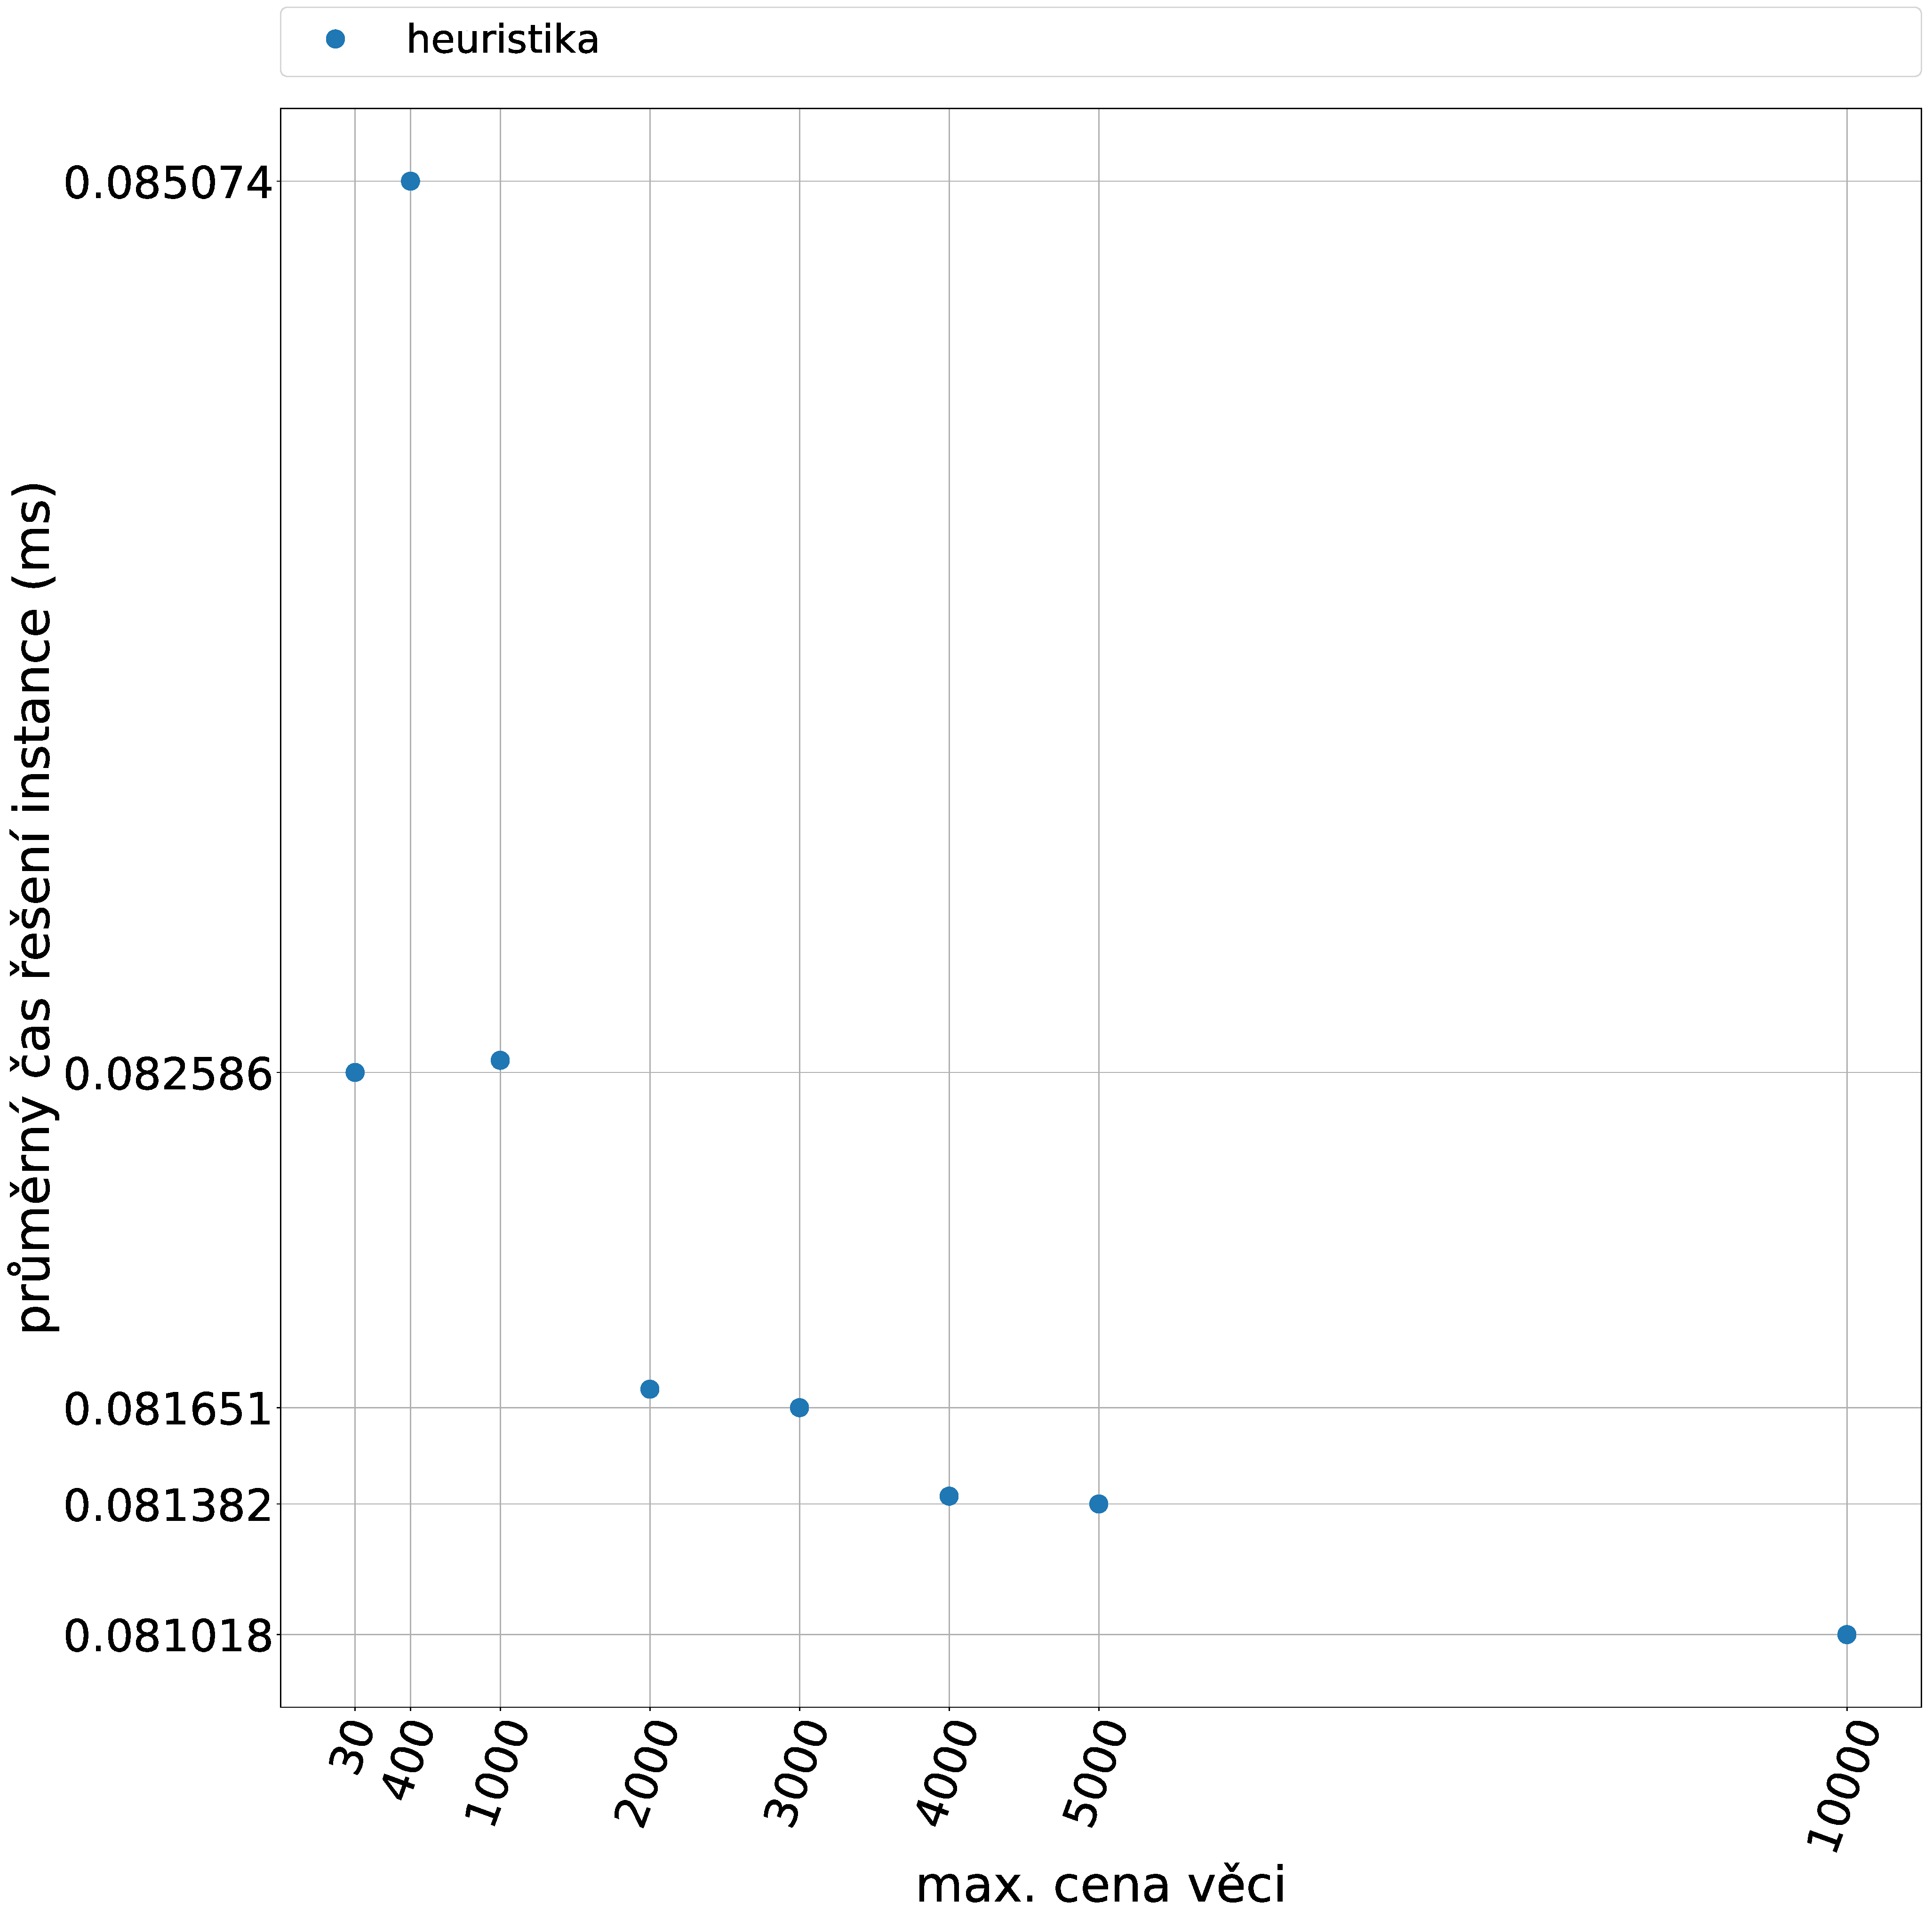
\includegraphics[width=\textwidth]{img/CH.pdf} 
    \end{minipage}
    \\
   \caption{Na grafech je ukázána vždy průměrná a maximální chyba heuristiky v závislosti na granularitě instance. Na levém grafu pro převahu malých instancí a na převém grafu pro převahu velkých instancí.}\label{fig:GOEI}
    \end{figure} 


\subsection{Závislost na maximální váze předmětů}

\begin{figure}
	\centering
    \begin{minipage}[c]{0.49\textwidth}
        \centering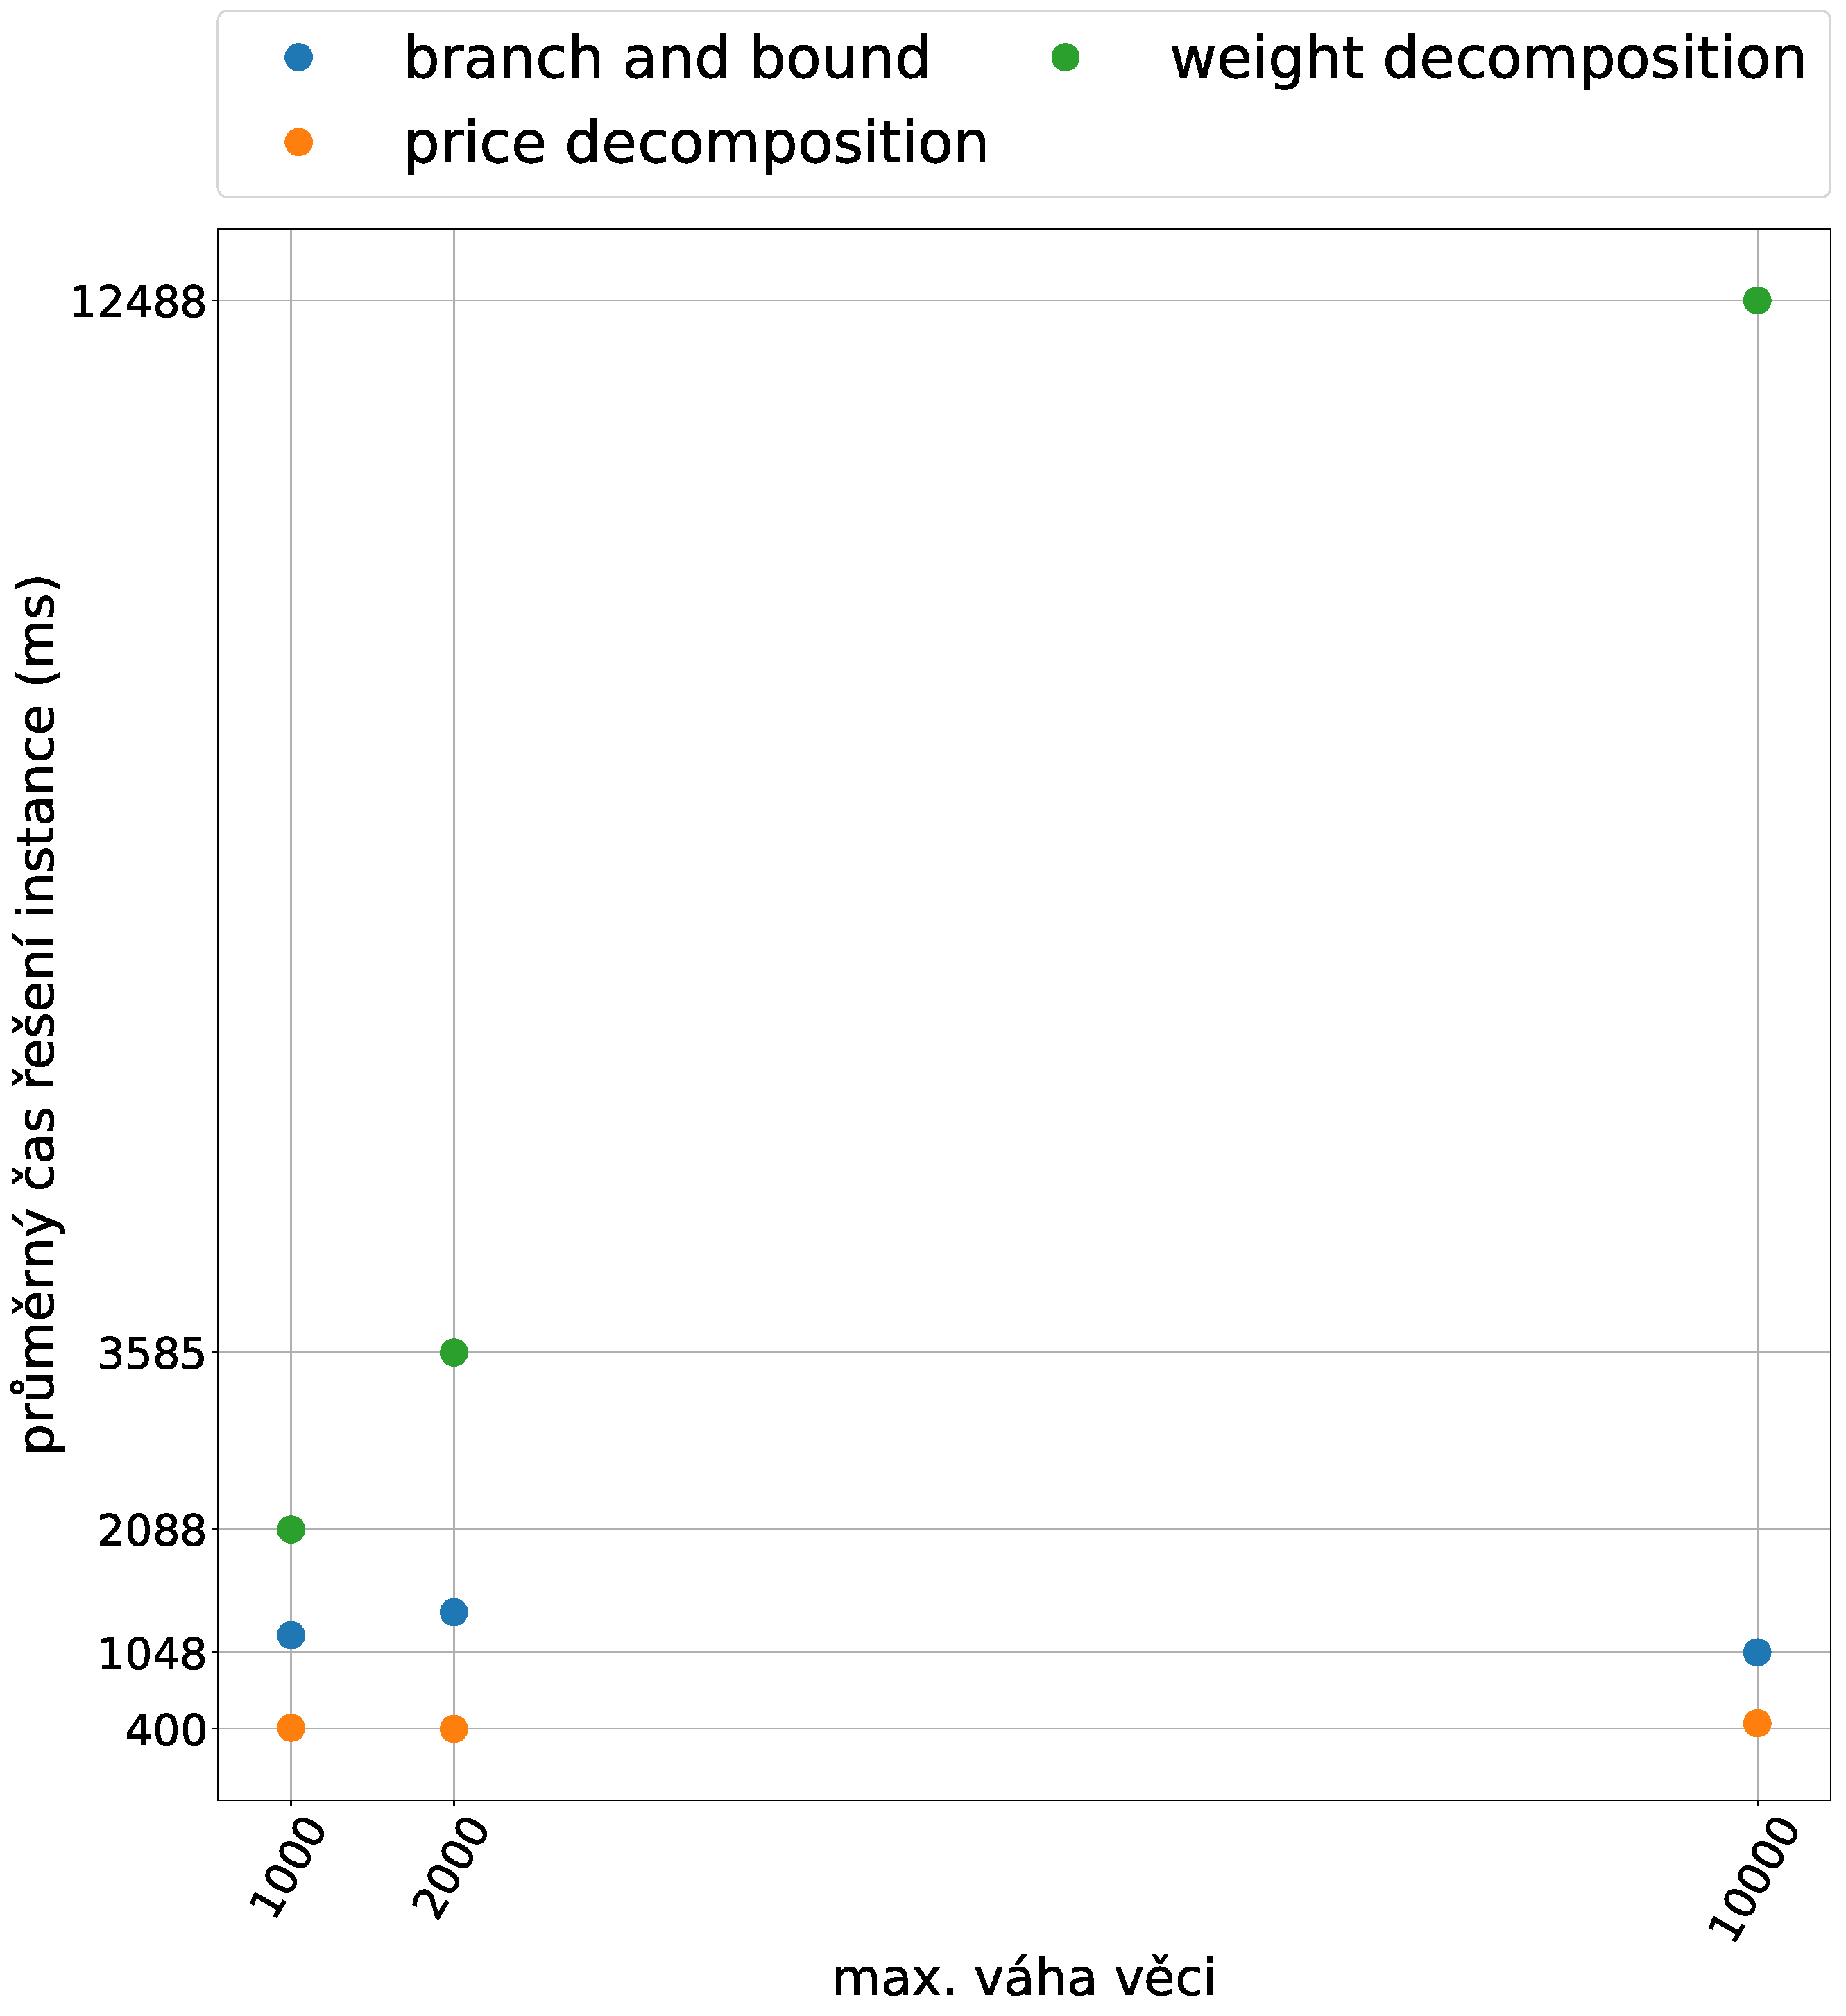
\includegraphics[width=\textwidth]{img/WE.pdf} 
    \end{minipage}
    \begin{minipage}[c]{0.49\textwidth}
        \centering 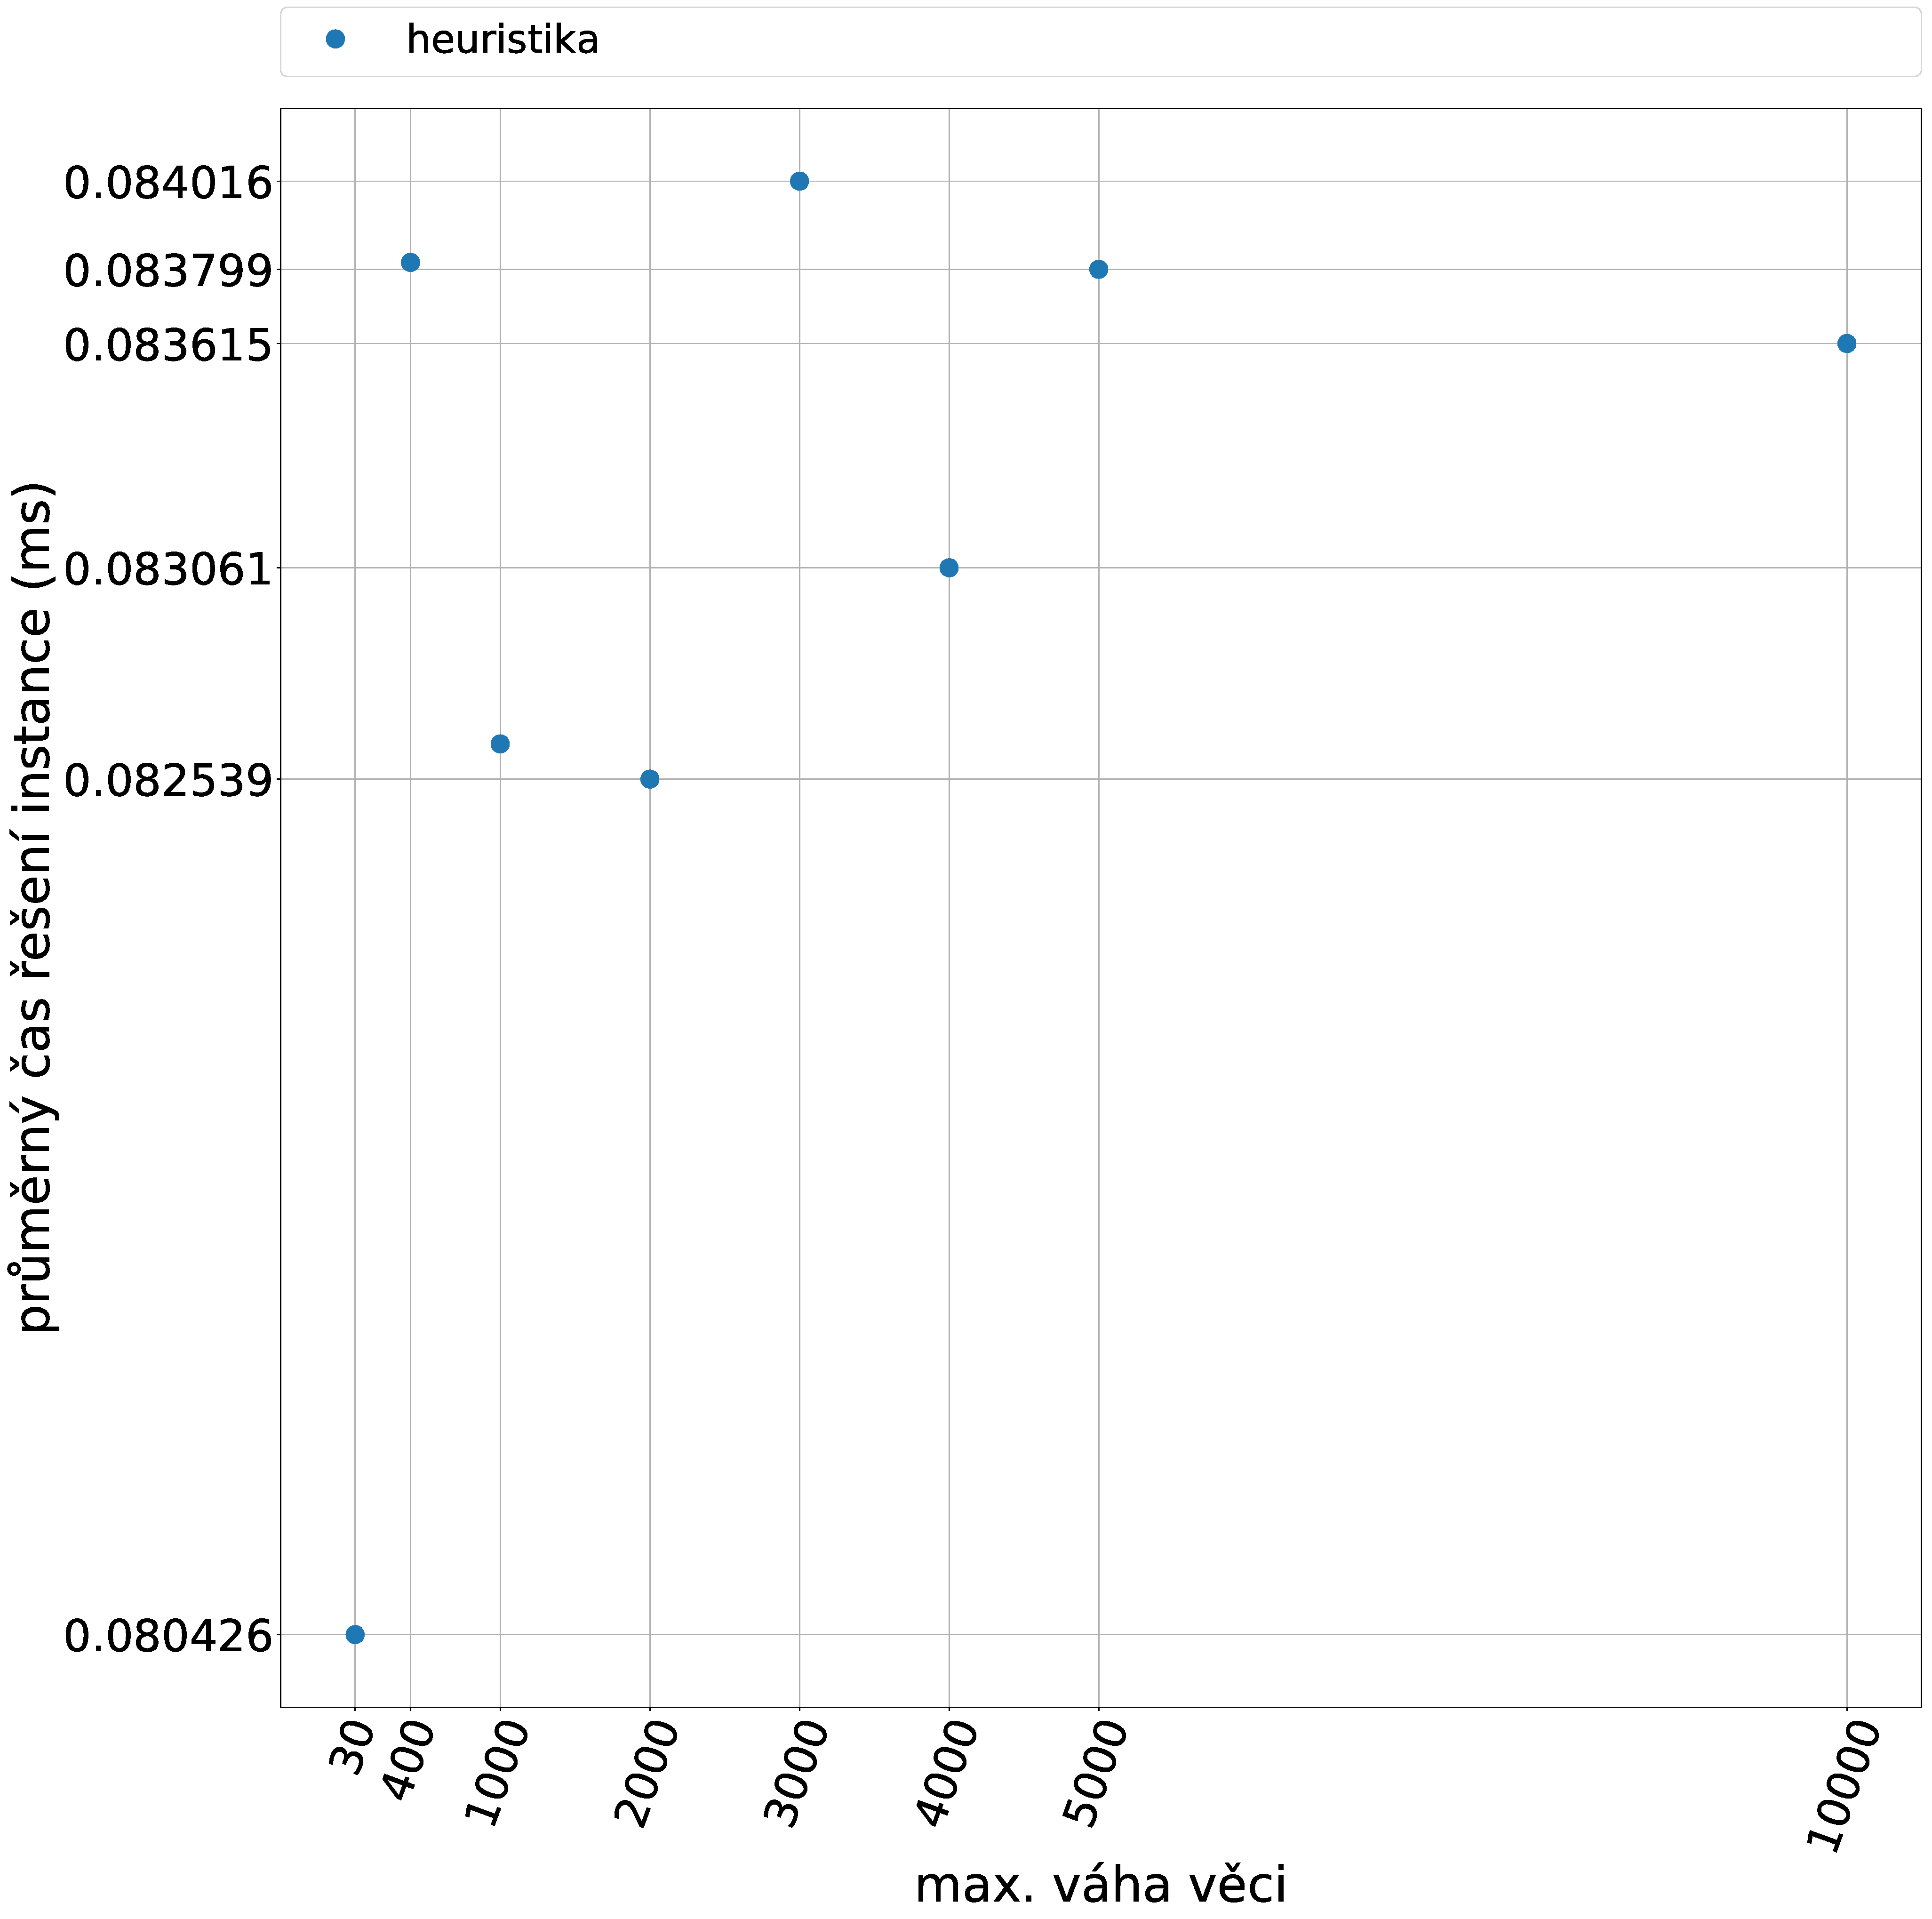
\includegraphics[width=\textwidth]{img/WH.pdf} 
    \end{minipage}
    \\
   \caption{Na grafech je ukázána vždy průměrná a maximální chyba heuristiky v závislosti na granularitě instance. Na levém grafu pro převahu malých instancí a na převém grafu pro převahu velkých instancí.}\label{fig:GOEI}
    \end{figure} 
        
    
\begin{figure}
	\centering
    \begin{minipage}[c]{0.49\textwidth}
        \centering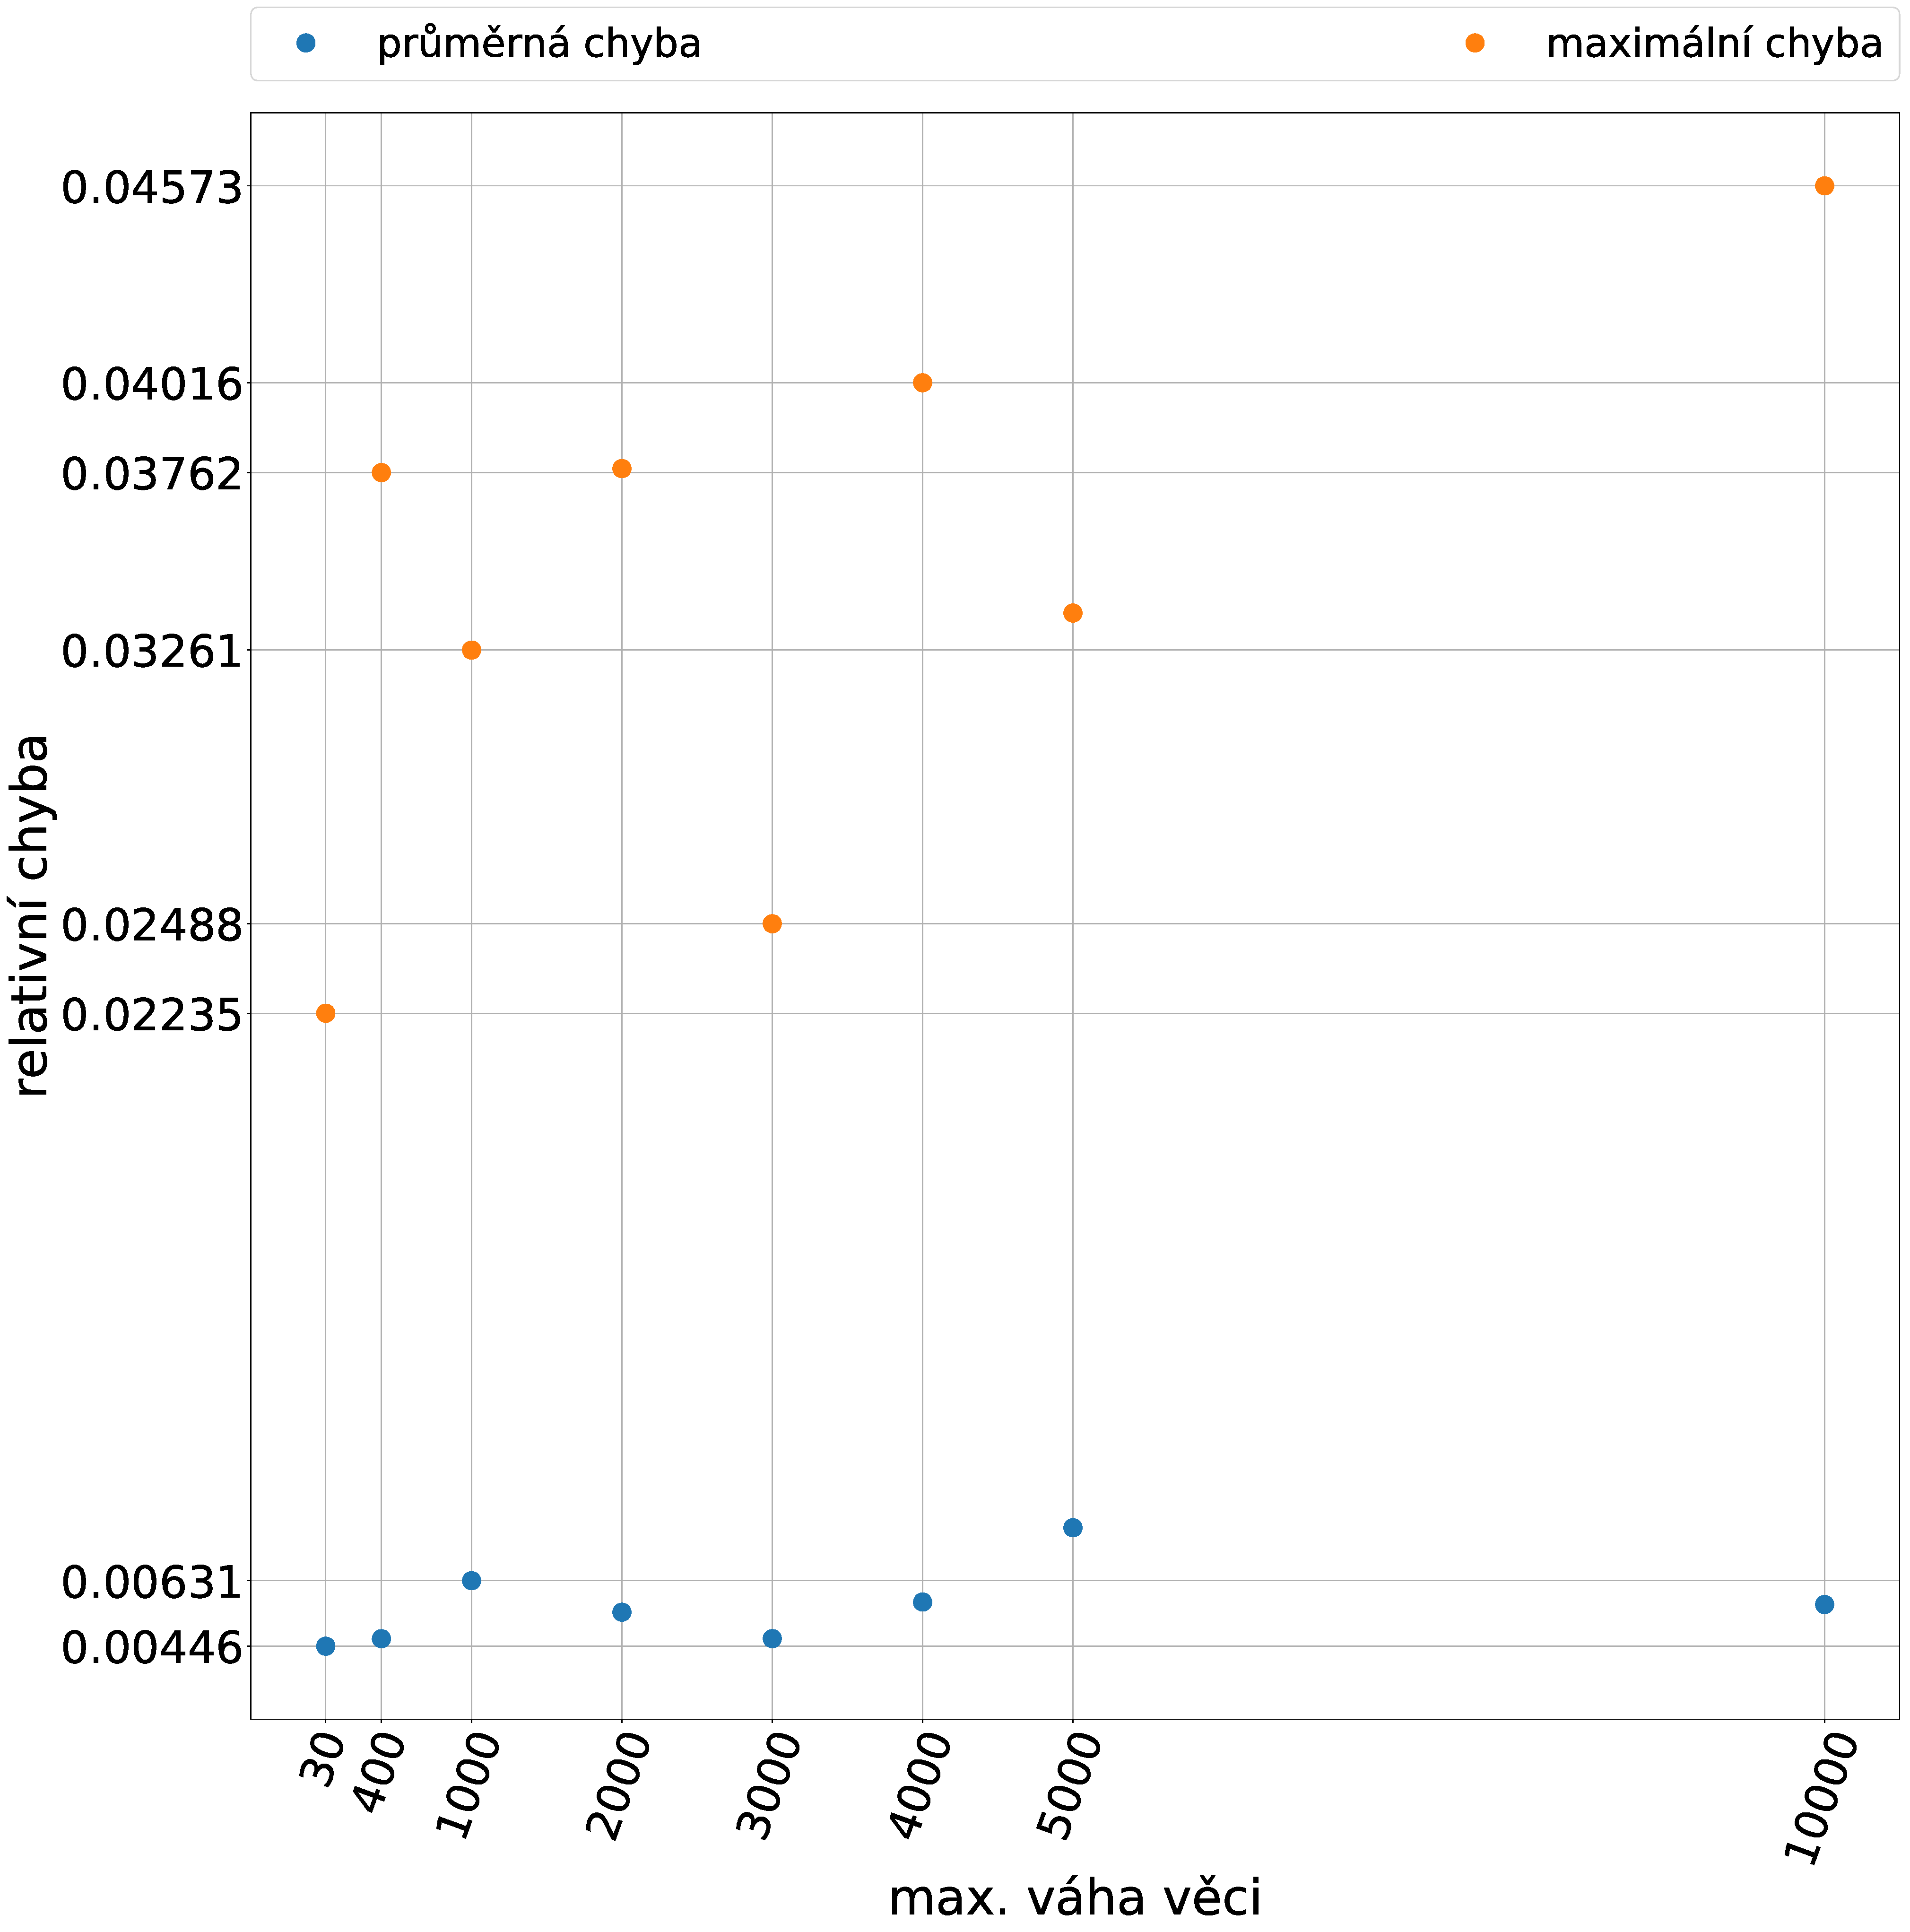
\includegraphics[width=\textwidth]{img/WHE.pdf} 
    \end{minipage}
    \begin{minipage}[c]{0.49\textwidth}
        \centering 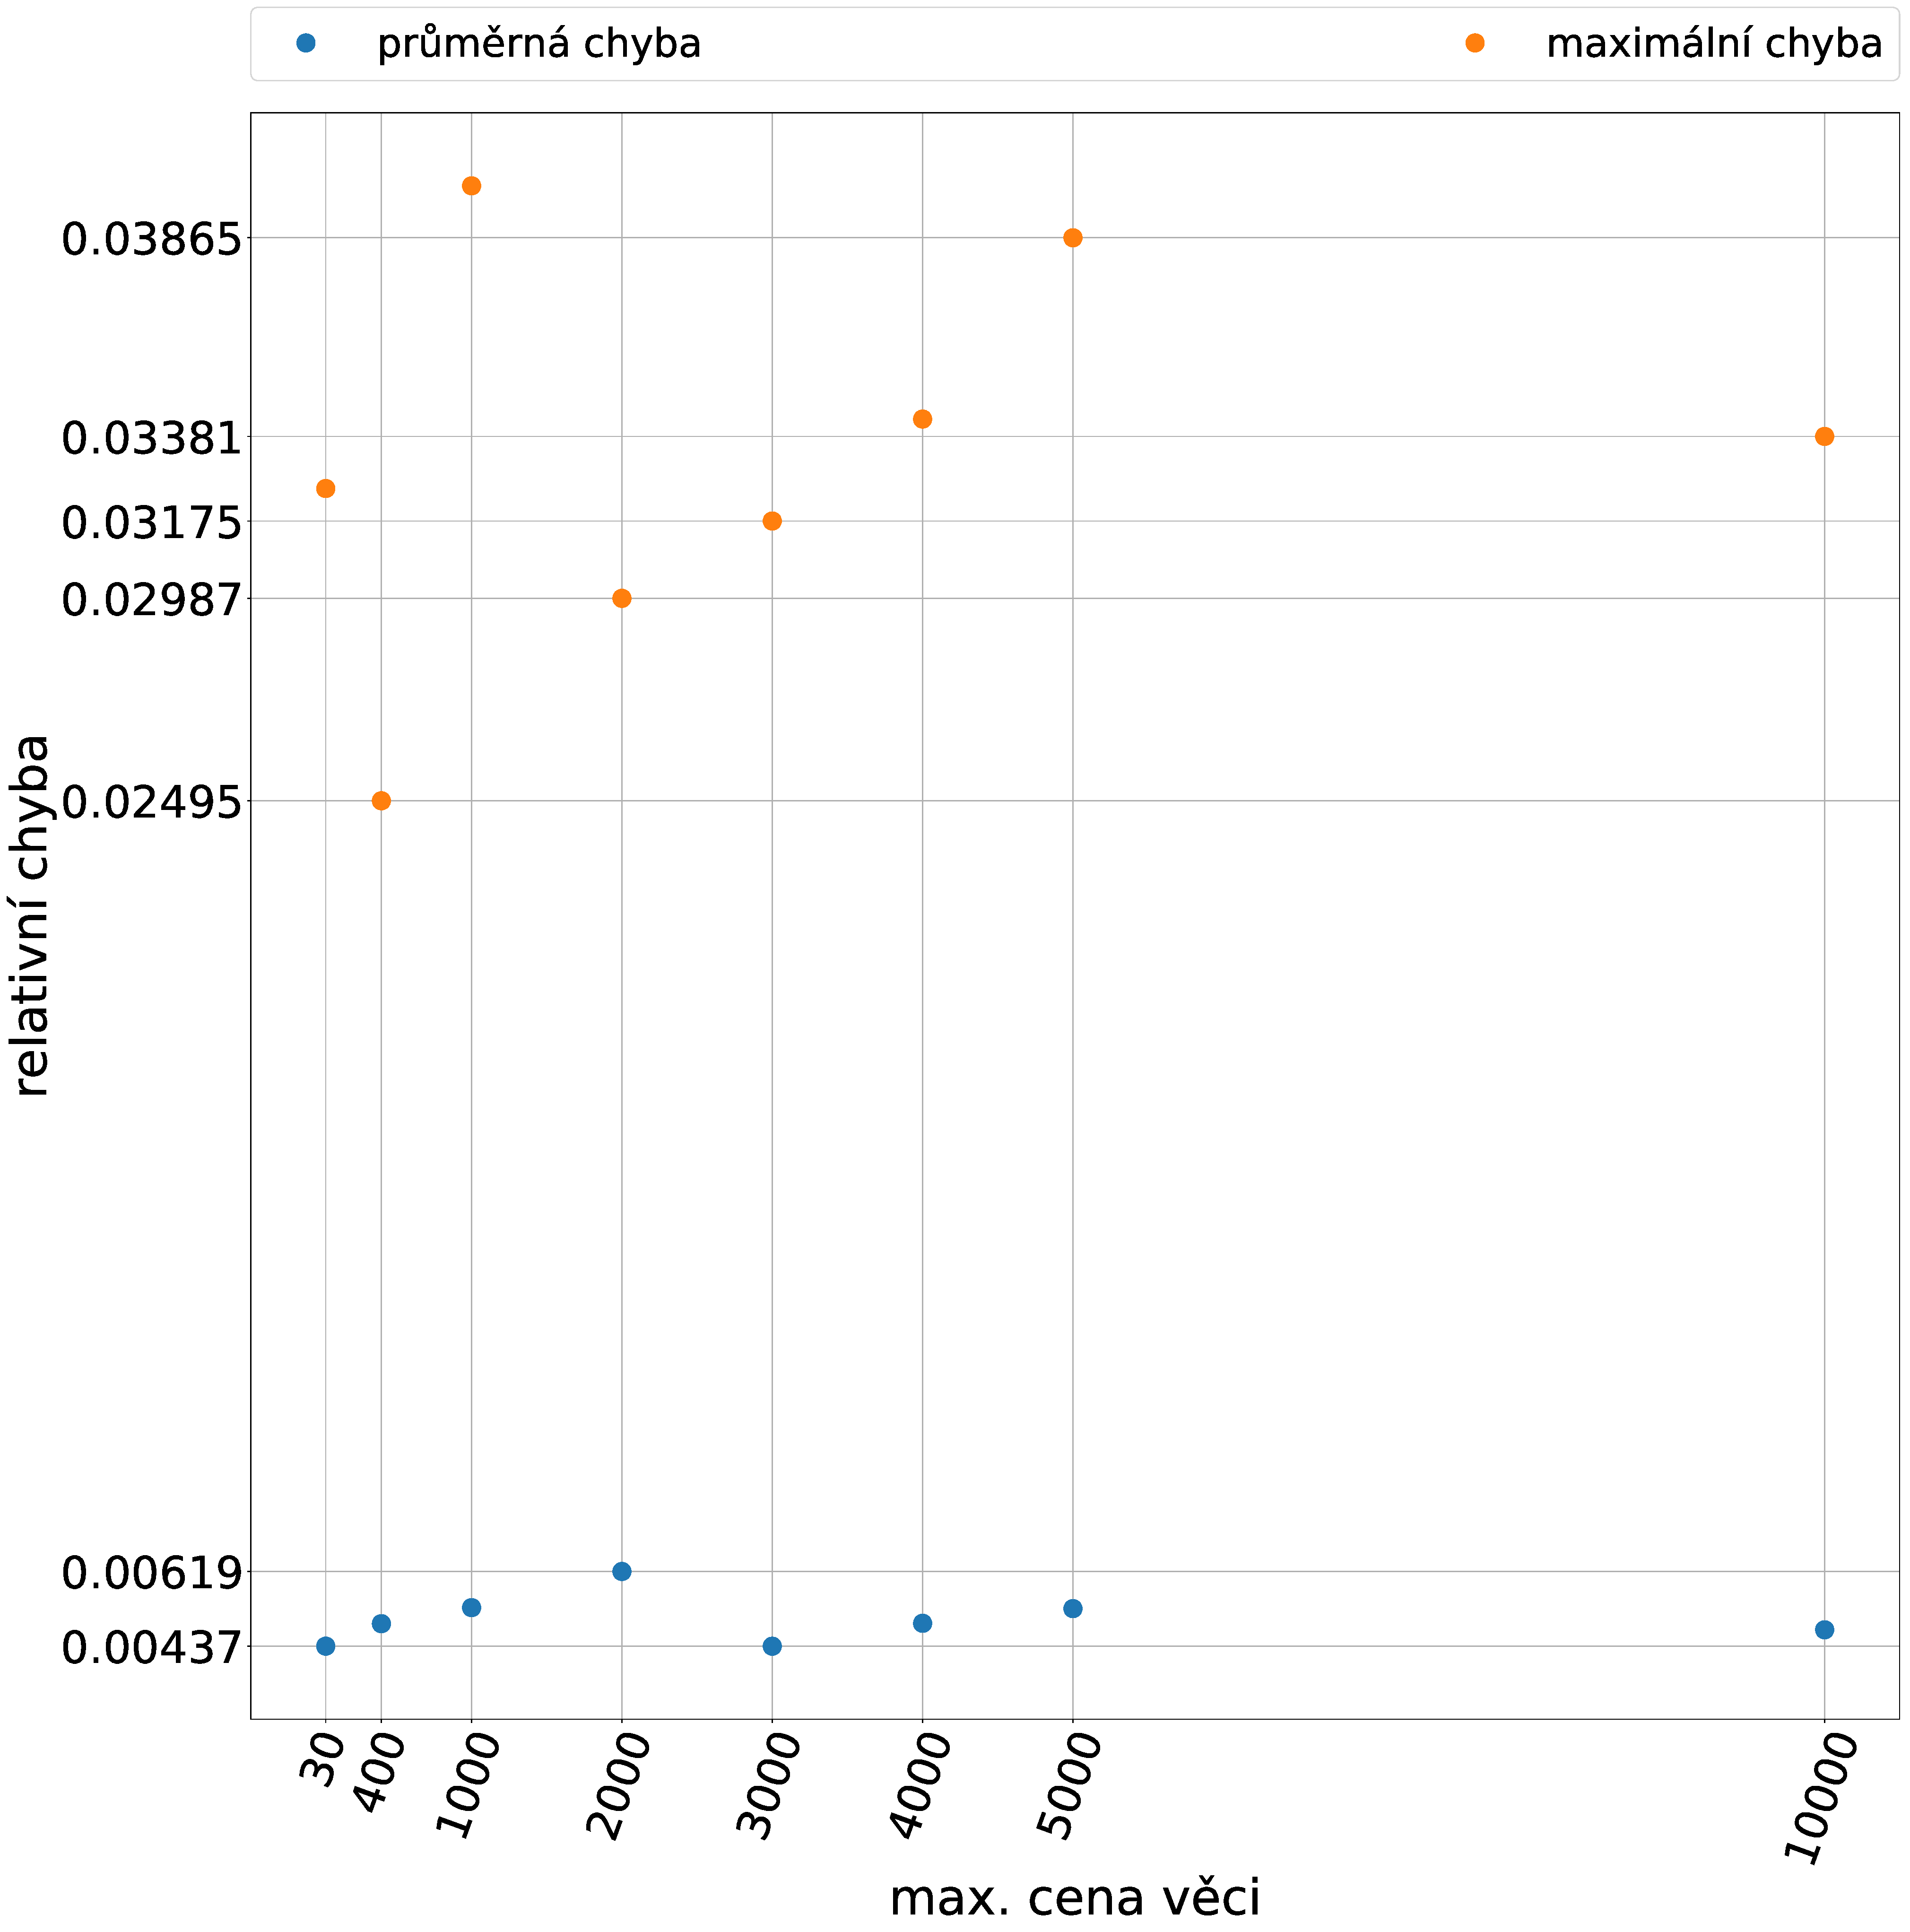
\includegraphics[width=\textwidth]{img/CHE.pdf} 
    \end{minipage}
    \\
   \caption{Na grafech je ukázána vždy průměrná a maximální chyba heuristiky v závislosti na granularitě instance. Na levém grafu pro převahu malých instancí a na převém grafu pro převahu velkých instancí.}\label{fig:GOEI}
    \end{figure} 
    
   




\section{Závěr}
Během experimentu jsem otestoval velké množství instancí s různými parametry a sledoval citlivost algoritmů na tyto parametry. Byli pozorovány časy exaktních algoritmů a u heuristiky byla také měřena relativní chyba. 


\end{document}